\chapter{HH4b: Background Estimate and Systematic Uncertainties}
\label{chap:six}

\section{Background Estimation\label{sec:BkgEst}}

\subsection{Alphabet Background Estimate\label{ss:Alphabet}}
After applying the kinematic selection, we define the ratio of multijet distributions that pass and fail the $\PH$ tagging requirement in data and QCD multijet MC simulation as $\rpfdata$ and $\rpfmc$, respectively. Because of the combinatorial nature of multijet processes, $\rpfdata$ and $\rpfmc$ are both smooth in the ($\mjred$,$\mred$) plane. The ratio of these ratios ($\rrat$) is then also smooth and can be used to correct for differences in simulation and data by parameterizing it with an analytic function. While $\rpfdata$ could also be described by an analytic function, it requires more parameters and a more complex shape relative to $\rrat$. The number of events in a given in bin in the passing category can then be estimated by:
\begin{equation}
    n_{\text{P,QCD}}(i) = n_{\text{F,QCD}}(i) \cdot \rpfmc \cdot \rrat,
    \label{eq:passDef}
\end{equation}
where $f(\mjred,\mred)$ has been replaced by $\rpfmc \cdot \rrat$ and $\rrat$ is a surface parameterized by a two-dimensional polynomial in the ($\mjred$,$\mred$) plane with coefficients whose values are a priori unknown to the fit. 
A second-order polynomial was chosen for the $\mred$ axis and the $\mjred$ axis. The parameters of the polynomials are uncorrelated between regions. 
To eliminate the effect of statistical fluctuations when calculating $\rpfmc$ in the QCD multijet simulation, pass and fail distributions are smoothed by using an adaptive kernel estimate~\cite{Cranmer2000KernelEI} (KDE). 
Figures \ref{fig:qcdsmoothingLL},\ref{fig:qcdsmoothingTT},\ref{fig:qcdsmoothing21} show the smoothed and un-smoothed distributions for $\rpfmc$. The mostly uniform distributions that we get after smoothing are what we expect 
because we are trying to factor out the statistical fluctuations in QCD due to low statistics. 
\begin{figure}[!htb]
	\centering
	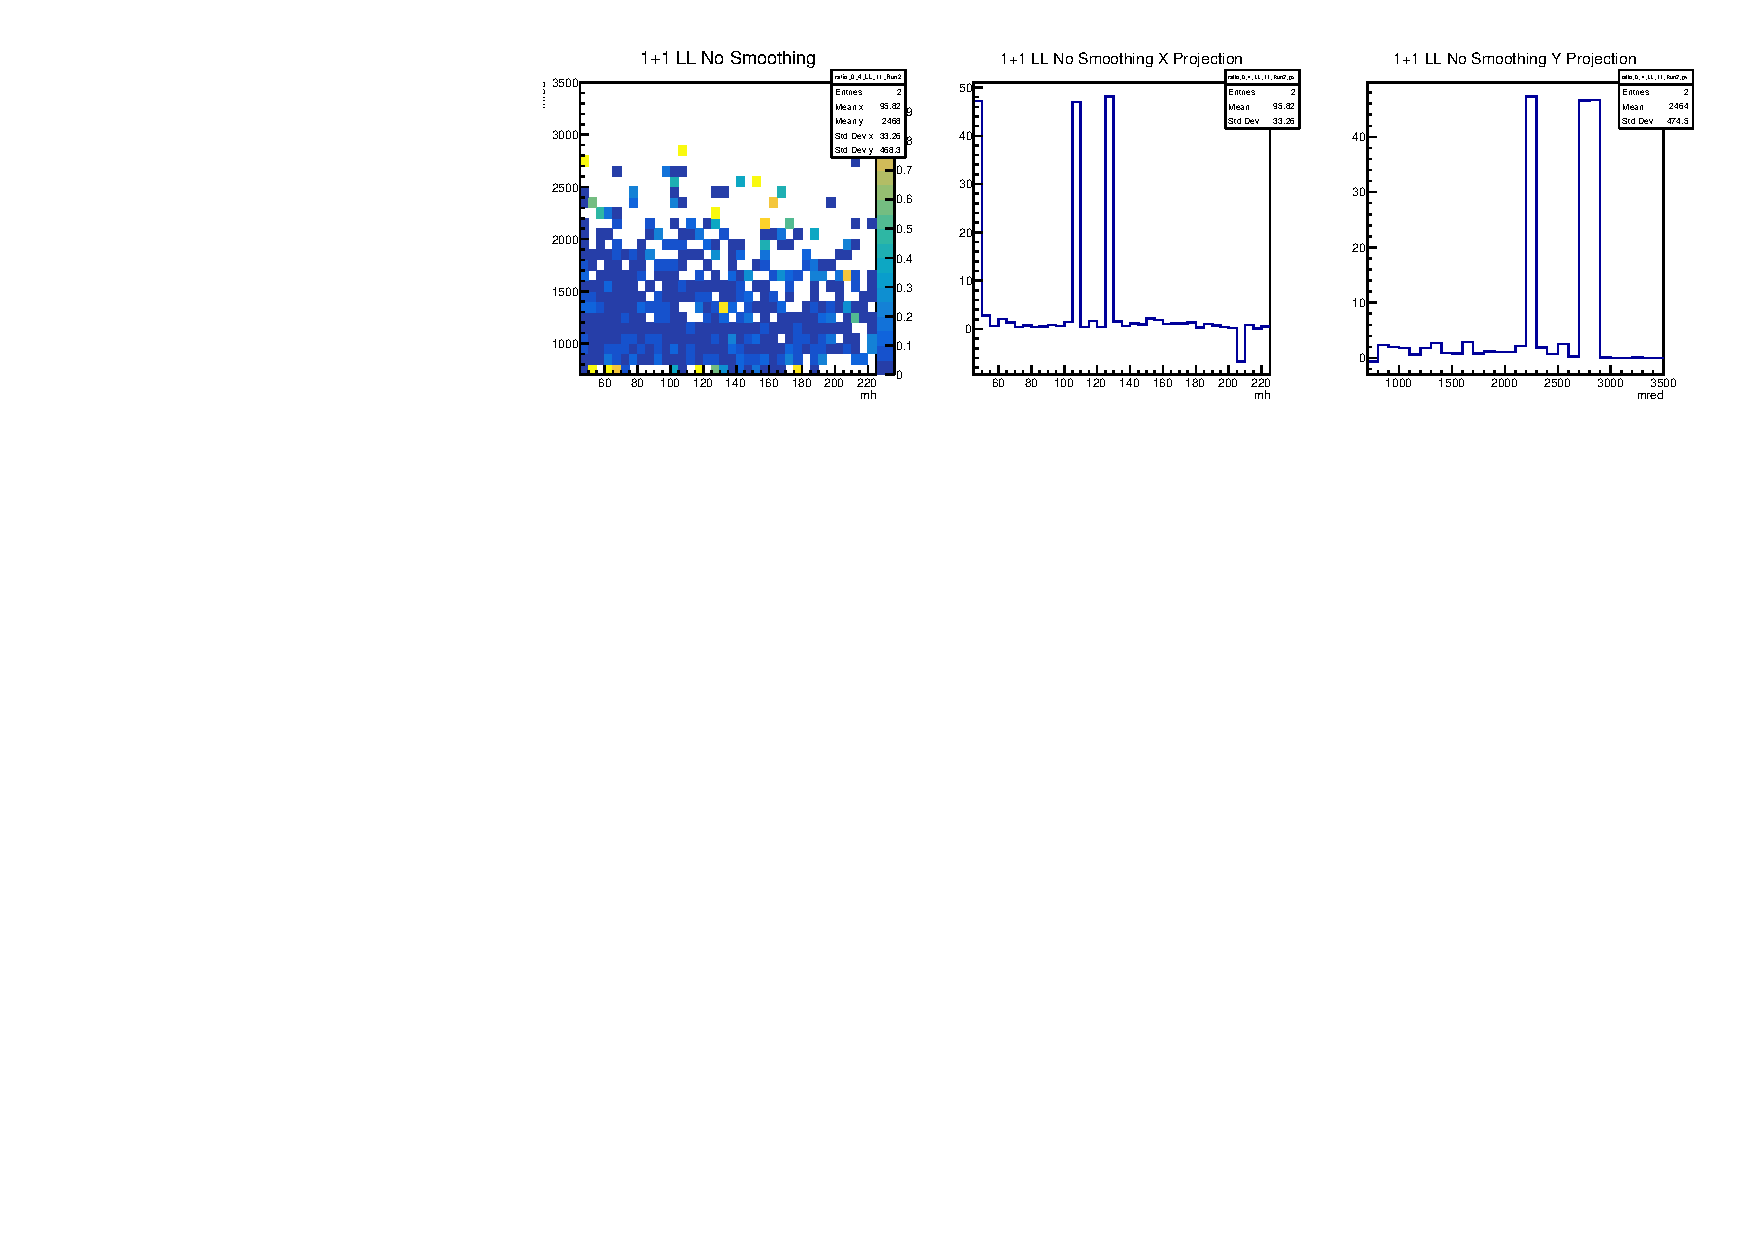
\includegraphics[width=1\textwidth]{Figures/LL_nosmoothing.pdf}
	\caption{Un-smoothed $\rpfmc$ distributions for Loose Loose.}
	\label{fig:qcdunsmoothingLL}
\end{figure}
\begin{figure}[!htb]
	\centering
	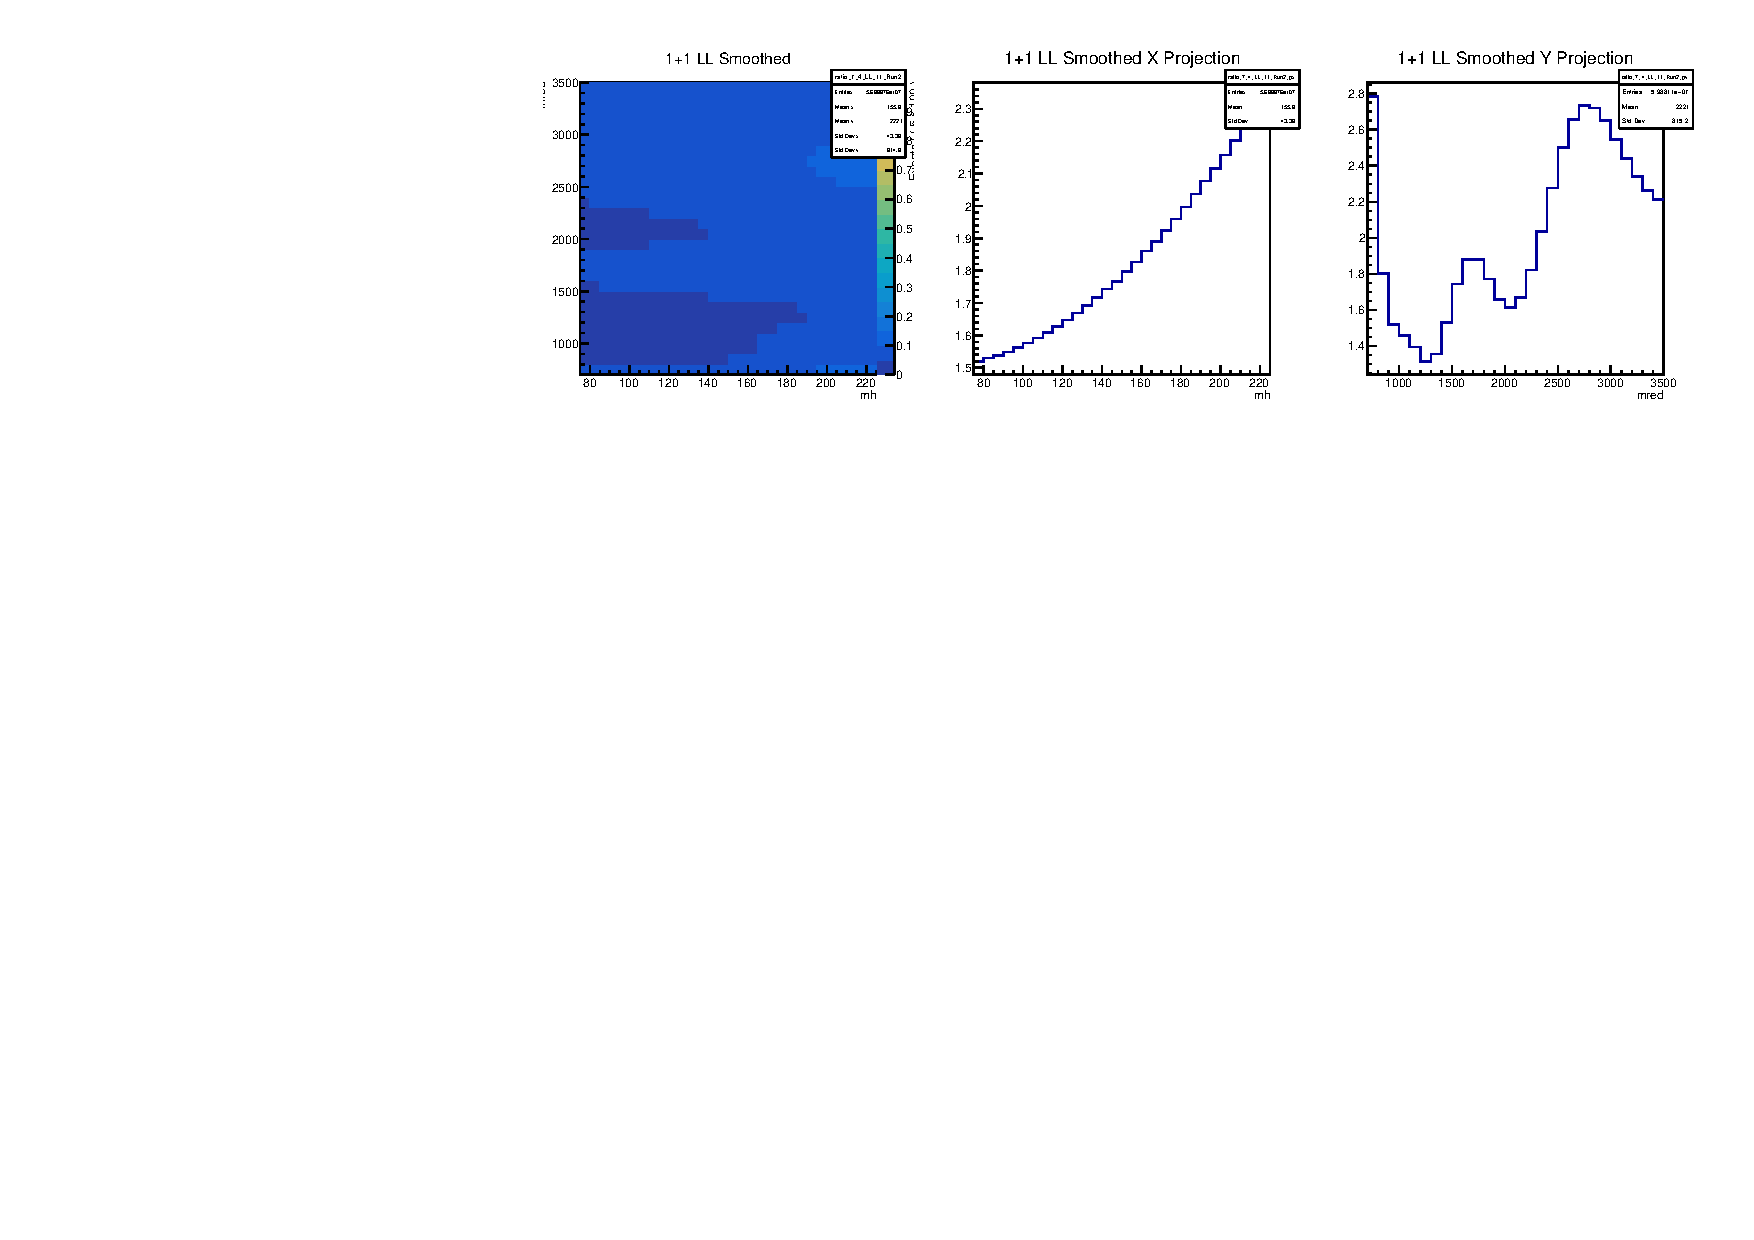
\includegraphics[width=1\textwidth]{Figures/LL_smoothed.pdf}
	\caption{Smoothed $\rpfmc$ distributions for Loose Loose.}
	\label{fig:qcdsmoothingLL}
\end{figure}
\begin{figure}[!htb]
	\centering
	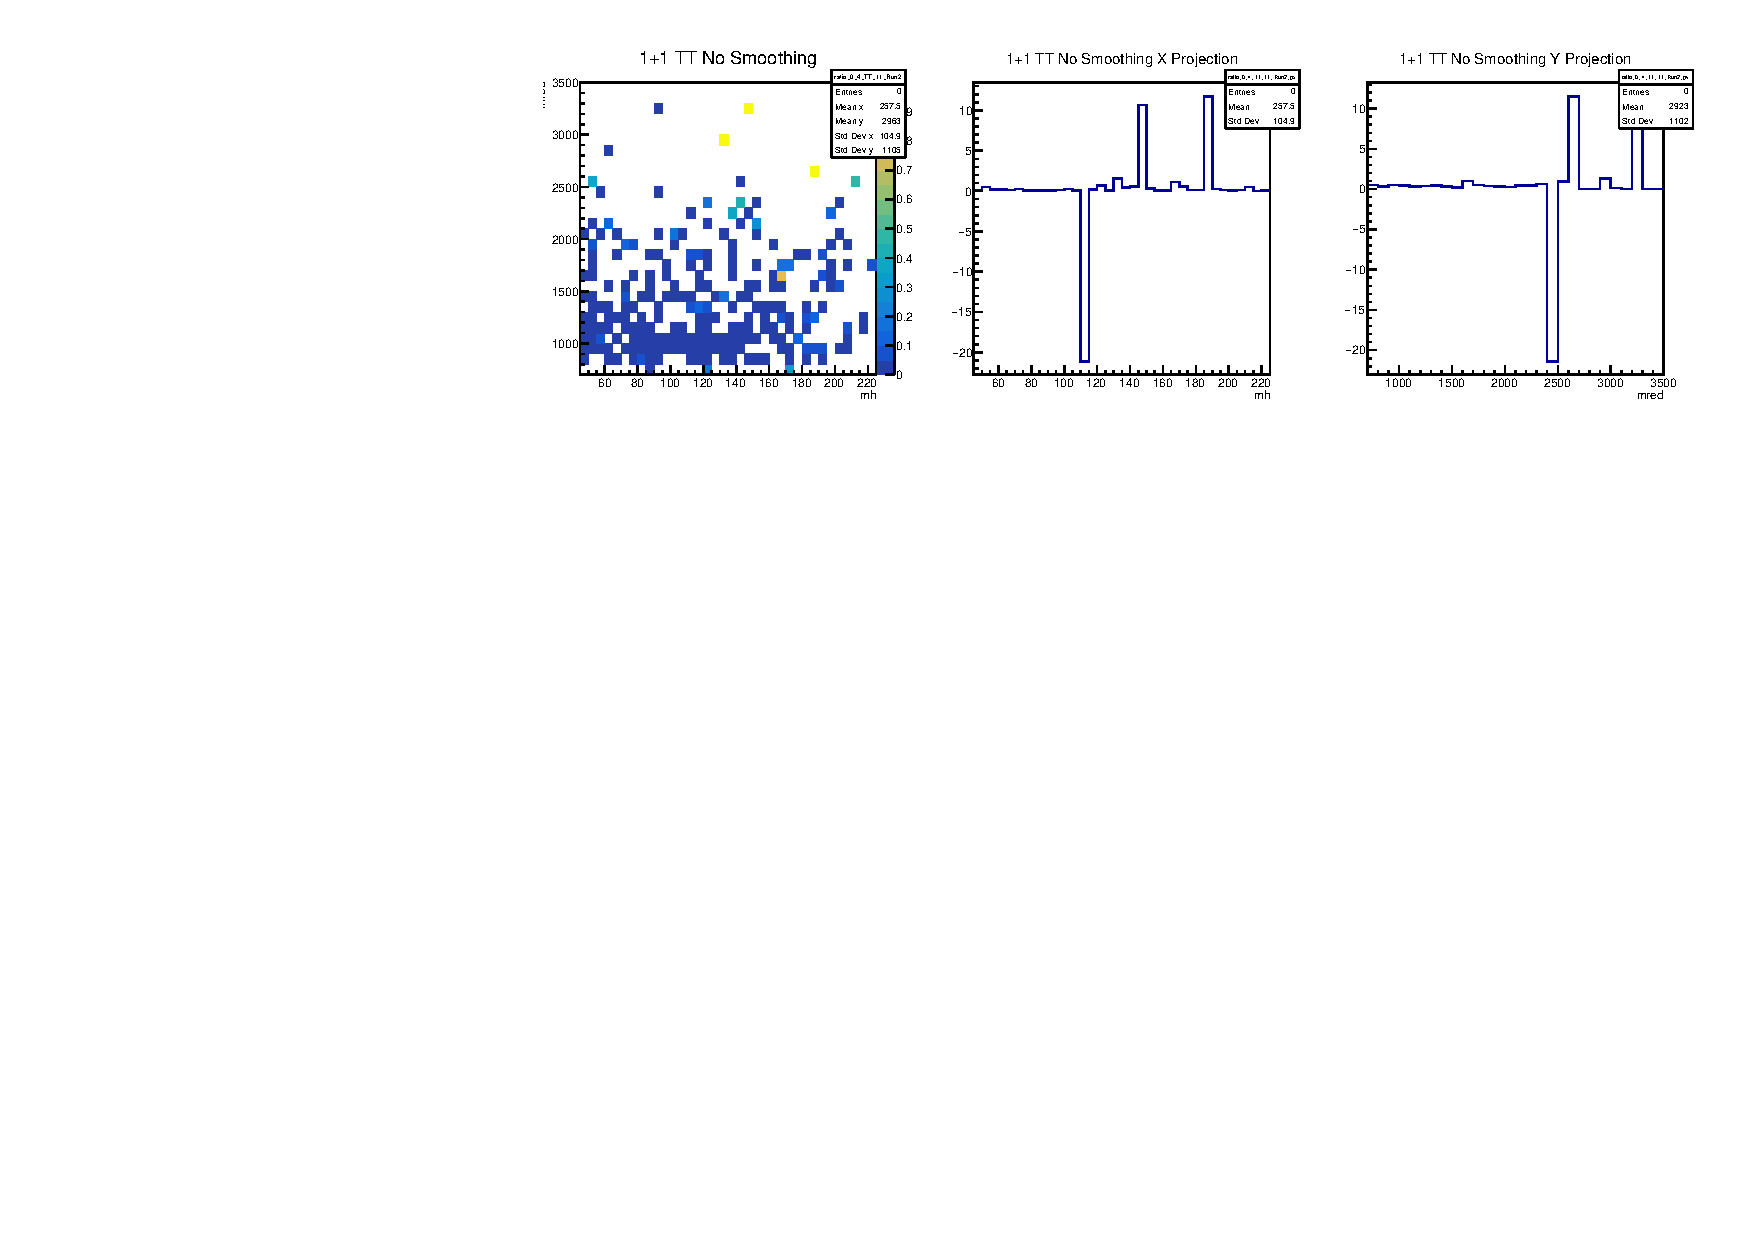
\includegraphics[width=1\textwidth]{Figures/TT_nosmoothing.pdf}
	\caption{Un-smoothed $\rpfmc$ distributions for Tight Tight.}
	\label{fig:qcdunsmoothingTT}
\end{figure}
\begin{figure}[!htb]
	\centering
	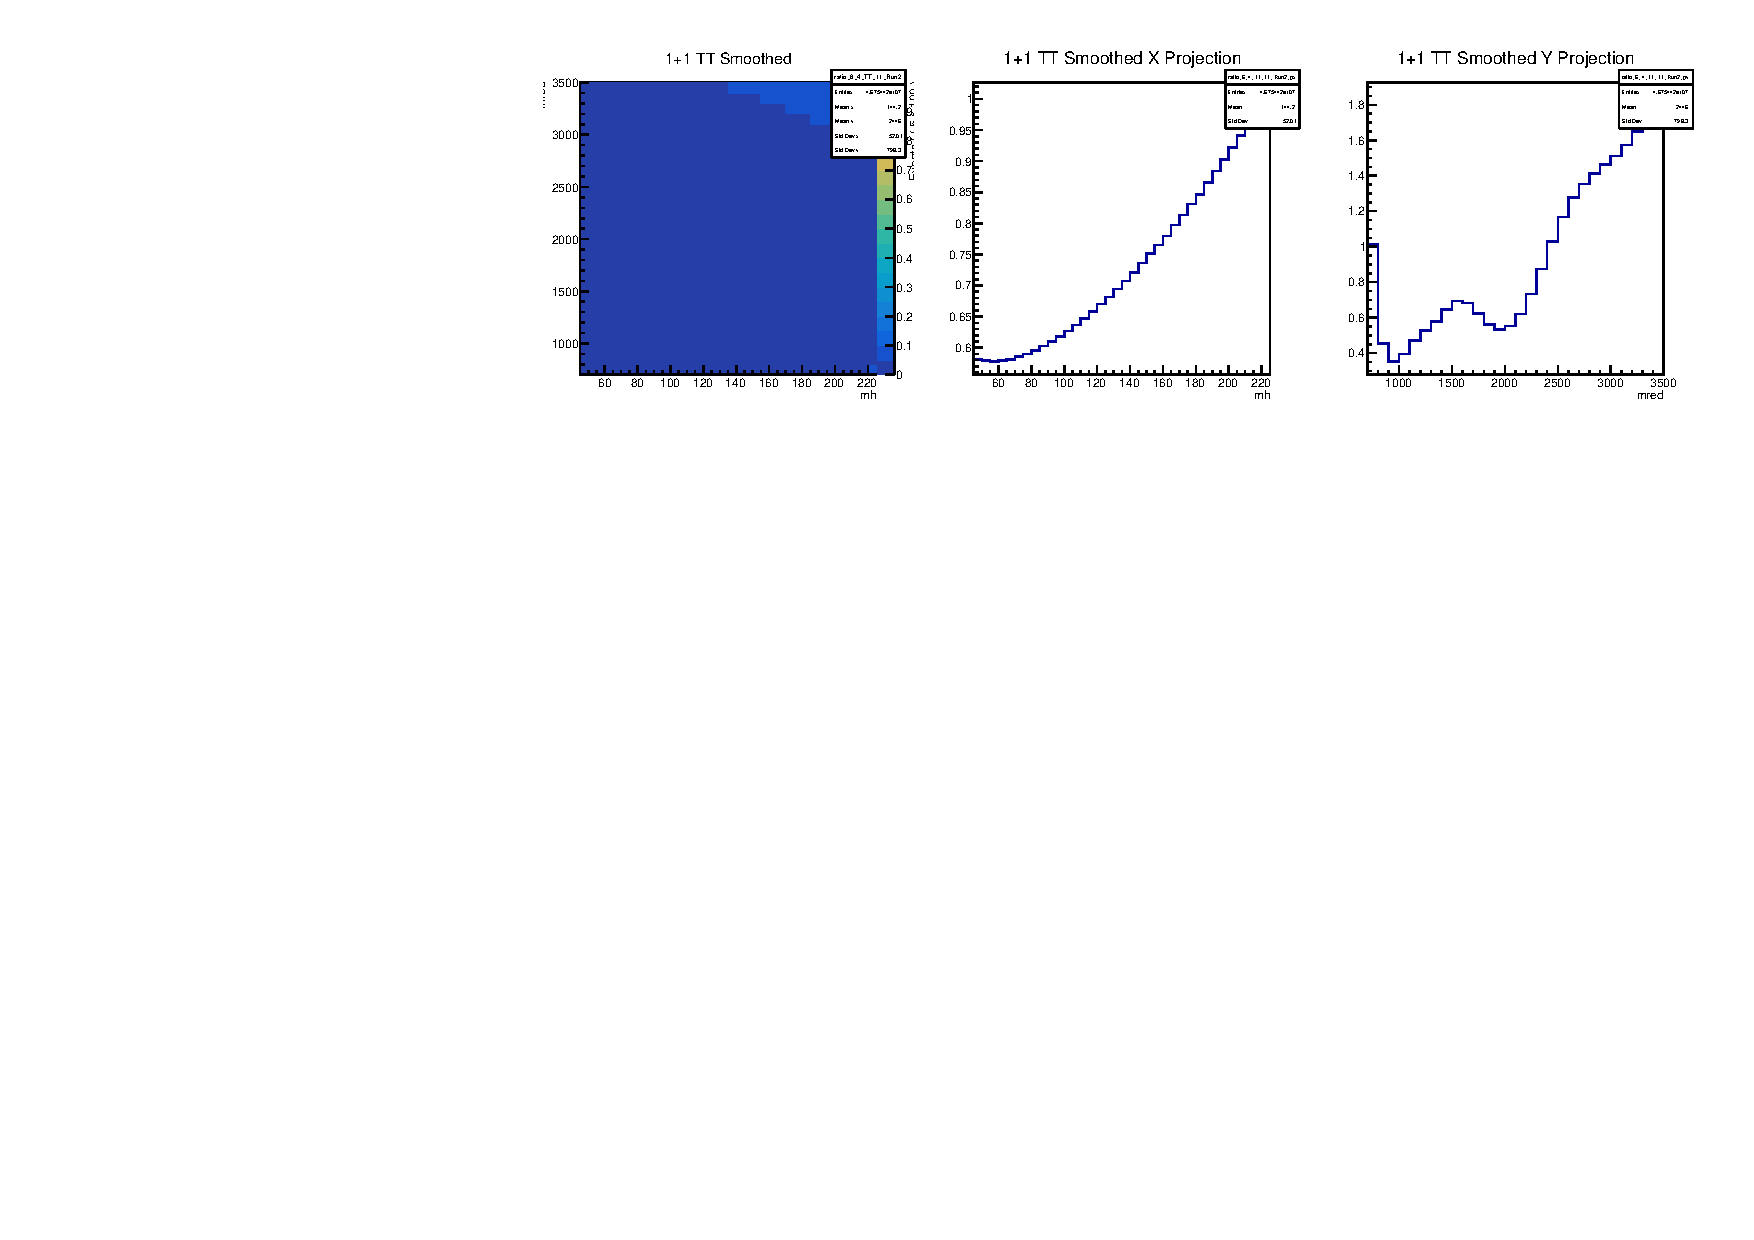
\includegraphics[width=1\textwidth]{Figures/TT_smoothed.pdf}
	\caption{Smoothed $\rpfmc$ distributions for Tight Tight.}
	\label{fig:qcdsmoothingTT}
\end{figure}
\begin{figure}[!htb]
	\centering
	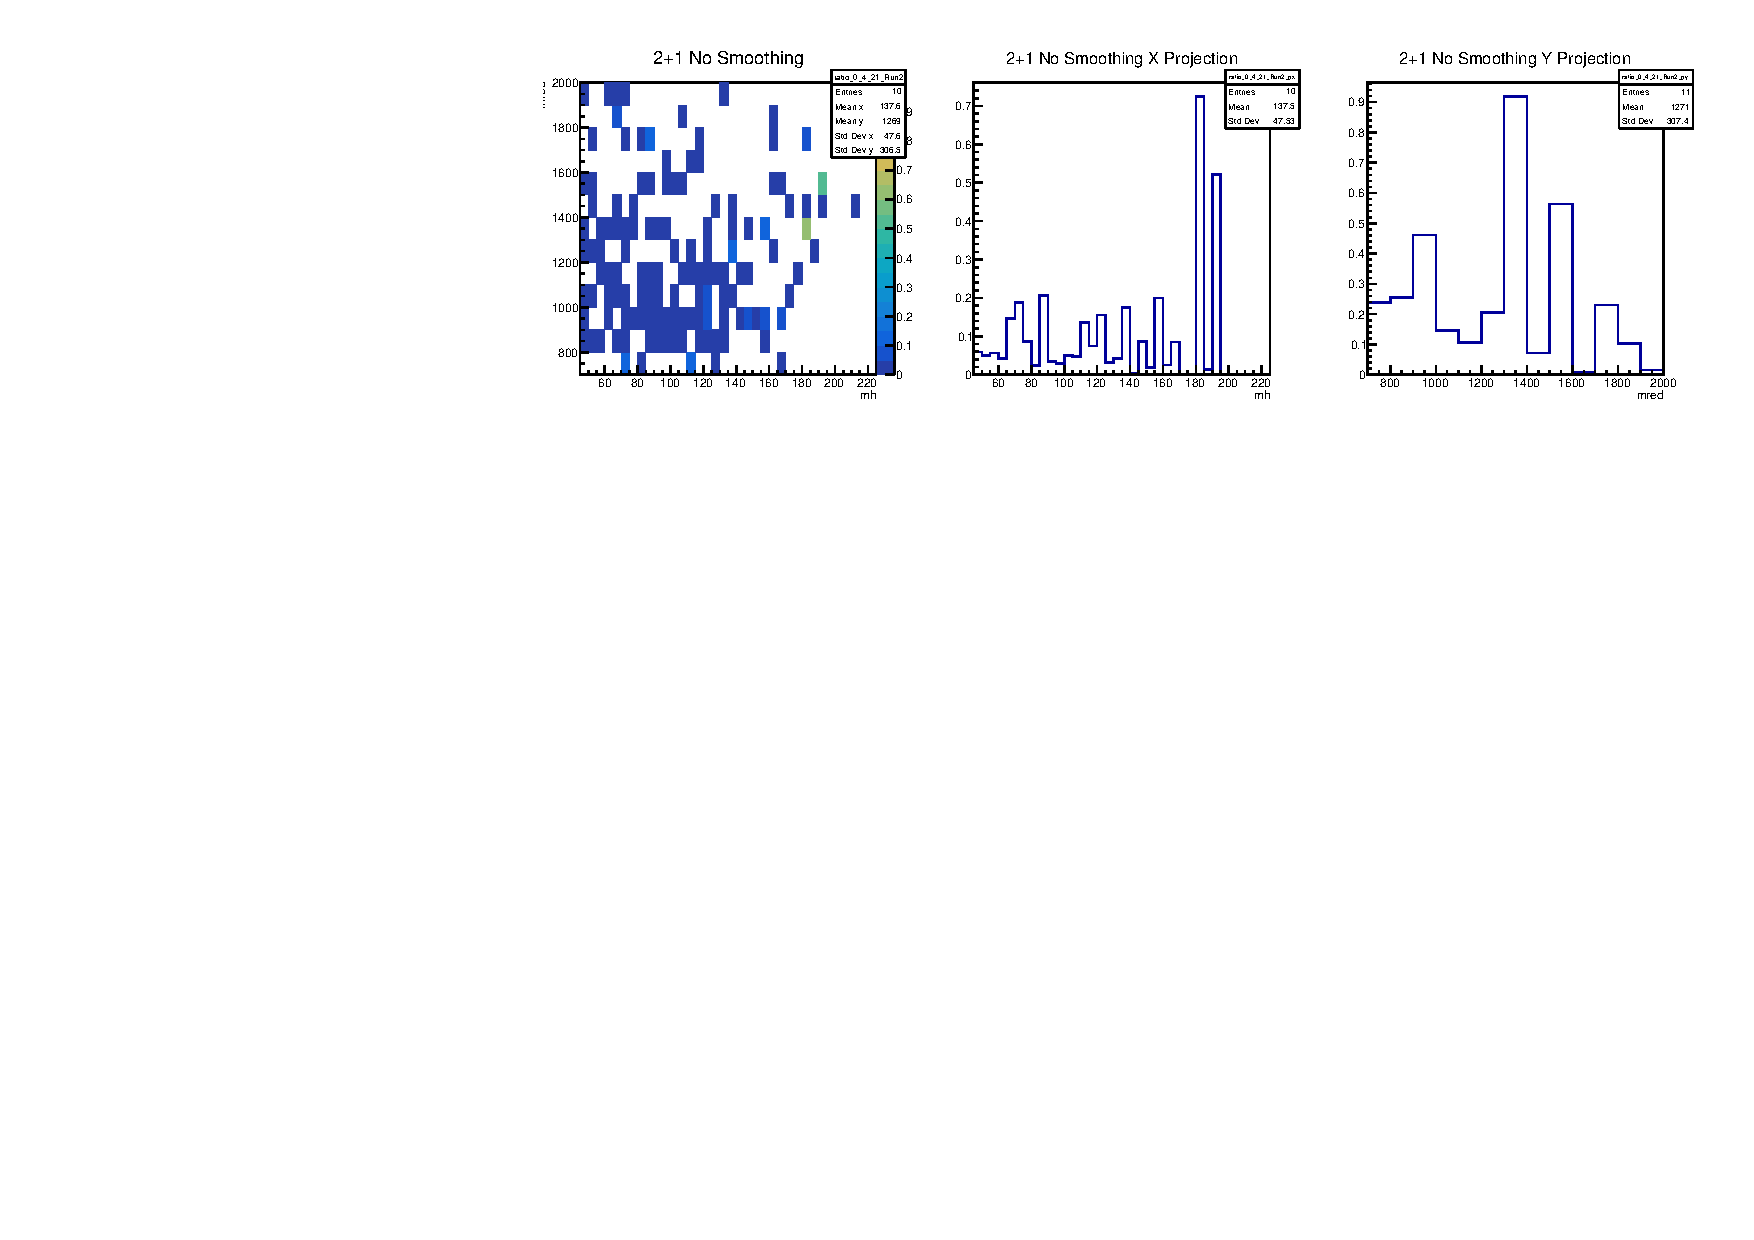
\includegraphics[width=1\textwidth]{Figures/21_nosmoothing.pdf}
	\caption{Un-smoothed $\rpfmc$ distributions for Semi-resolved.}
	\label{fig:qcdunsmoothing21}
\end{figure}
\begin{figure}[!htb]
	\centering
	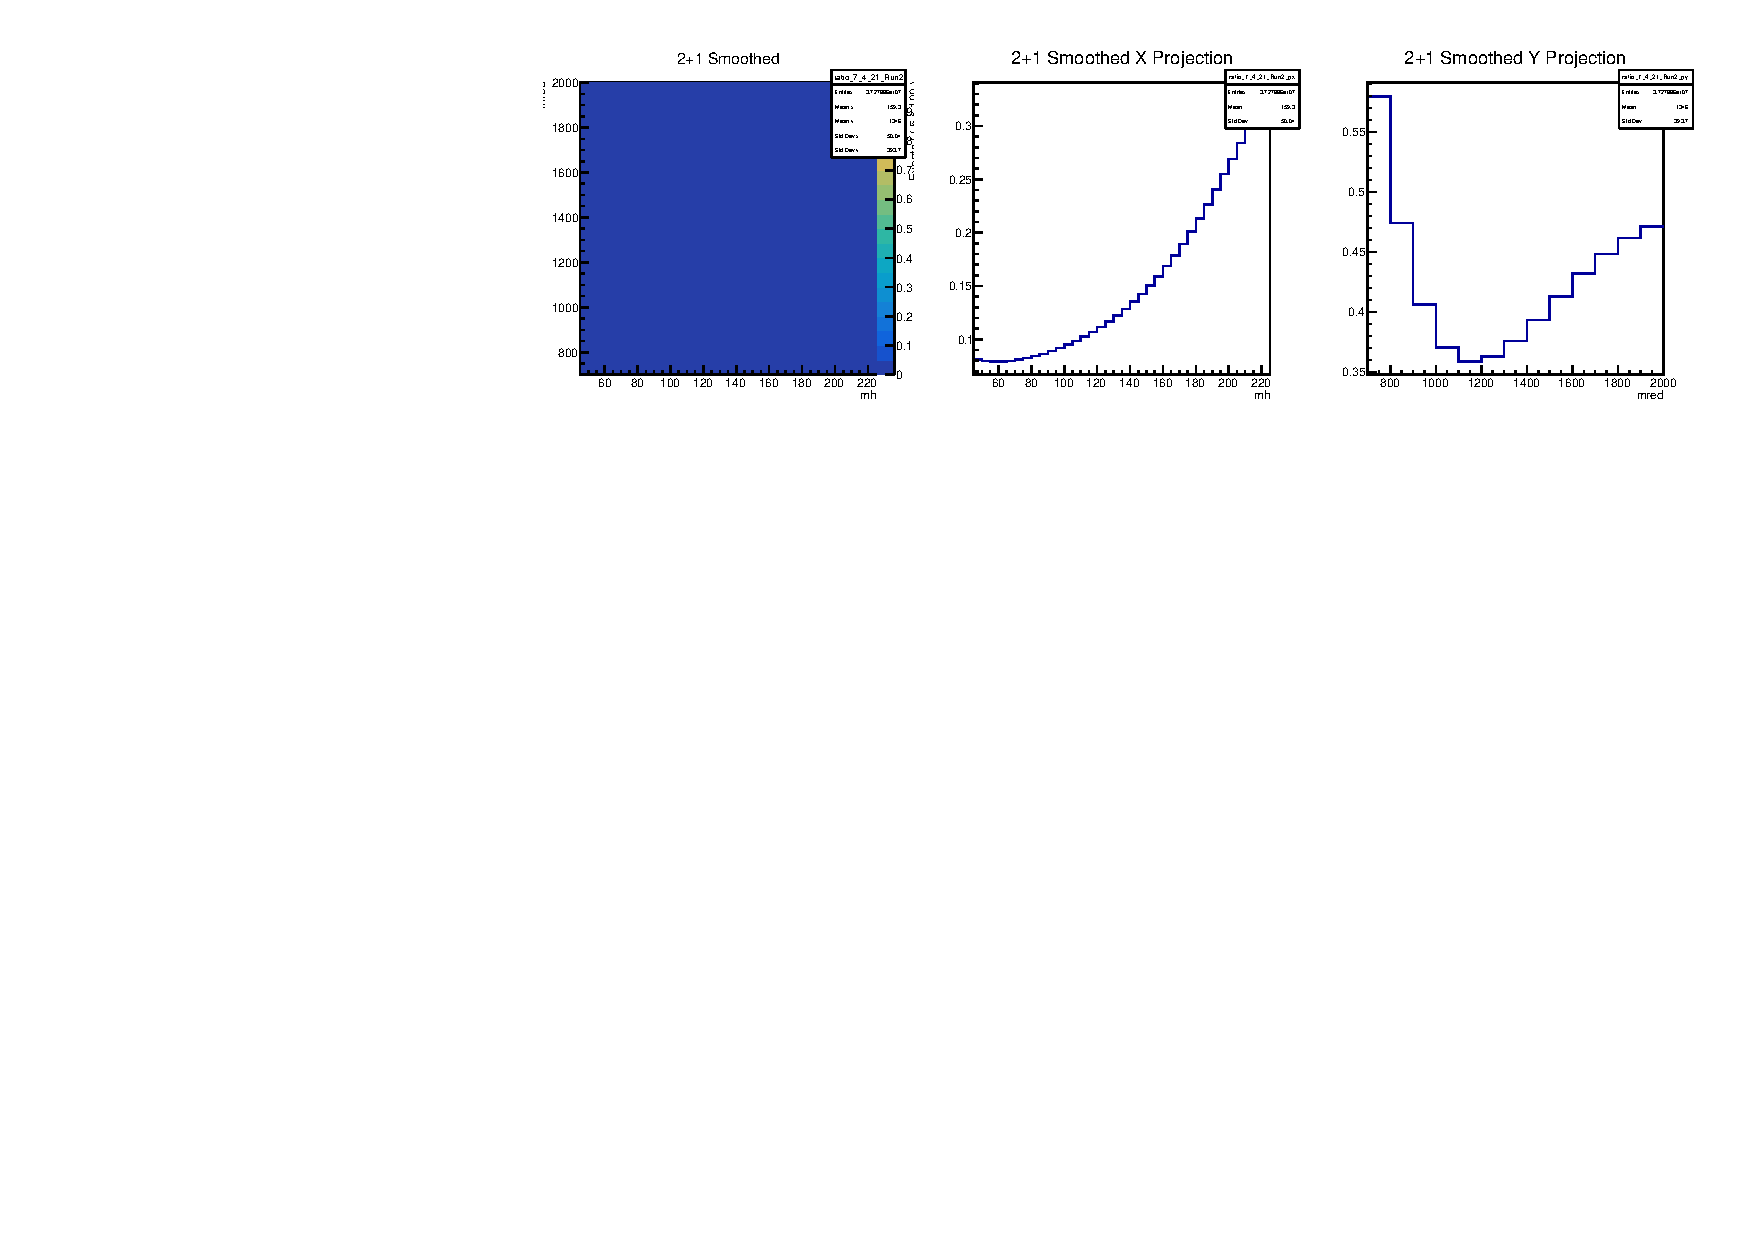
\includegraphics[width=1\textwidth]{Figures/21_smoothed.pdf}
	\caption{Smoothed $\rpfmc$ distributions for Semi-resolved.}
	\label{fig:qcdsmoothing21}
\end{figure}

\clearpage
Due to the fact that the QCD MC samples are binned in HT, they need to be normalized to each other's cross sections before they are combined. While also normalizing to data luminosity, samples could be scaled by factors between 0.15 and 8.43. These have significant impacts on the effective yield per-bin passed to the Kernel Density Estimate and can thus change the bandwidth of the kernels which adapts to the statistics per-bin. Since we want to smooth based on the generated statistics, a KDE PDF is built per HT-bin and samples \textit{before} the scaling and stitching. One billion events are generated for the pass and fail distribution of each HT-binned sample and then normalized to the relative cross sections and data luminosity. The KDE generated distributions are then stitched to together and the ratio of pass and fail is taken to create the $\rpfmc$. We also perform the same smoothing with the $\ttbar$ distributions in order to eliminate any statistical fluctuations that cause the fit to try to enhance an un-physical peak.  
Two parameters $\rho$ and $\sigma$ control the smoothing as follows. $\rho$ is a scale factor that is applied to the bandwidth calculated for each kernel. $\sigma$ determines the size of the box that is used to search for contributing kernels around a given point and is also used for the 1st non-adaptive pass for the calculation of adaptive keys pdfs. The various values for the KDE bandwidth, $\rho$ and $\sigma$, are shown here:
\begin{center}
\begin{tabular}{ |c|c| } 
 \hline
 Region & Features  \\ 
 \hline
 TT & QCD $\rho$ = 6 and $\sigma$ = 4, $\ttbar$ $\rho$ = 1 and $\sigma$ = 2\\ 
 LL & QCD $\rho$ = 7 and $\sigma$ = 4, $\ttbar$ $\rho$ = 1 and $\sigma$ = 2\\ 
 2+1 & QCD $\rho$ = 7 and $\sigma$ = 4, $\ttbar$ $\rho$ = 1  and $\sigma$ = 2\\   
 \hline
\end{tabular}
\end{center}
% Let us define the ratio of two-dimensional ($M_j$ vs $M_{jj}^{red}$) events of pass and fail multijet distributions in data as $R_{P/F} (M_j, M_{jj}^{red})$. This is a smooth surface in the ($M_j$ ,$M^{red}_{jj}$) plane and accounts for differences between data and simulation. To estimate the passing distribution in data, $n_P^{\rm data}(M_j, M_{jj}^{red})$, one can multiply the failing distribution in data, $n_F (data)$ ($M_j$ ,$M^{red}_{jj}$) , by $R_{P/F}$. 
% \begin{equation}
% n_P^{\rm data}(M_j, M_{jj}^{red}) = n_F^{\rm data} (M_j ,M^{red}_{jj}) \times R_{P/F}
% \end{equation}
% We use this method by calculating $R_{P/F}$ explicitly. The analysis is blinded, so this fit is performed with the Higgs mass signal region masked from the fit. Specific to this analysis and the 2D Alphabet method is the new RooParametricHist2D class that was designed as a 2D version of RooParametricHist class from the Combine package. The use of RooParametricHist2D is necessary for the QCD background estimate because it allows each bin in the two dimensional object to float so that both the shape and normalization of the QCD background estimates in the pass and fail distributions can be determined. The failing QCD distribution bins are initialized to the data in that bin minus the nominal (not floating) non-QCD background MC values in that bin. However, these failing QCD bins are allowed to float over a large range relative to their nominal value during the fit and float without penalty to the likelihood so that they may freely change in value. This ensures that, if any non-QCD MC morphs during the fit, the QCD bins can accommodate without explicitly needing to know which backgrounds changed and by how much. The fit function give for $R_{P/F}$ is a 2nd order polynomial in both dimensions. 

\subsubsection{Fitting procedure\label{Fitting}}
The production cross section of $\sigma(\Pp\Pp \to X \to \HH \to \bbbar \bbbar)$ is evaluated by
comparing for each bin in the two-dimensional ($\mjred$,$\mred$) distribution, the number of
observed and expected events, given the expected background and the theoretical cross section. The expected number of events is calculated as
$N_{\textrm{expected}} = \sigma_{\HH \to \bbbar \bbbar} \times \varepsilon \times \mathcal{L}$, where $\sigma_{\HH \to \bbbar \bbbar}$ is the $\HH \to \bbbar \bbbar$ cross-section, $\varepsilon$ is the acceptance times the efficiency, and $\emph{L}$ is the integrated luminosity of our dataset. A likelihood fit to data is used to test the signal hypothesis where the total background model is constructed as a sum of the individual background contributions using a Poisson model for each bin of the ($\mjred$, $\mred$) distribution. The number of expected failing and passing events in a given bin $i$ is given by
\begin{align}
n_{\text{F}}(i,\vec{\theta}) &= n_{\text{F}}^{\text{QCD}}(i) + n_{\text{F}}^{\ttbar}(i,\vec{p}) + n_{\text{F}}^{\text{signal}}(i,\vec{r})\\
& \nonumber \text{and} \\
n_{\text{P}}(i,\vec{\theta}) &= n_{\text{P}}^{\text{QCD}}(i) + n_{\text{P}}^{\ttbar}(i,\vec{p}) + n_{\text{P}}^{\text{signal}}(i,\vec{r}),
\end{align}
where $i$ is a bin in the ($\mj$,$\mred$) plane, $\vec{p}$, $\vec{q}$, and $\vec{r}$ are the nuisance parameters, and $\vec{\theta}$ is the union set of all nuisance parameters. The variable $n_{i,\text{F,QCD}}$ is an unconstrained positive real number. Finally, $n_{\text{P,QCD}}(i)$ is given by
\begin{equation}
    n_{\text{P,QCD}}(i) = n_{\text{F,QCD}}(i) \cdot f(\mjred,\mred),%\rpfmc \cdot \rrat,
    \label{eq:passDef2}
\end{equation}
where $f(\mjred,\mred)$ is a transfer function used in the data-driven multijet background estimate and described fully in Section \ref{ss:Alphabet}. The negative log-likelihood is then
\begin{equation}\label{eq:nLL}
\begin{split}
-\ln L(\vec{d};\vec{\theta}) =
    \sum_{i=1}^{N_{\text{bins,F}}} \left[n_{\text{F}}(i,\vec{\theta}) - d_{\text{F}}(i) \ln n_{\text{F}}(i,\vec{\theta}) + \ln d_{\text{F}}(i) ! \right]\\
    + \sum_{i=1}^{N_{\text{bins,P}}} \left[(n_{\text{P}}(i,\vec{\theta}) - d_{\text{P}}(i) \ln n_{\text{P}}(i,\vec{\theta}) + \ln d_{\text{P}}(i) !)\right],
\end{split}
\end{equation}
where $N_{\text{bins,F}}$ and $N_{\text{bins,P}}$ are the total number of bins in the fail and pass distributions, respectively, and $d_{i,\text{F}}$ and $d_{i,\text{P}}$ are the number of observed events in a given bin in the fail and pass distributions, respectively.
% The production cross section of $\sigma(\Pp\Pp \to X \to \HH \to \bbbar \bbbar)$ is evaluated by comparing for each bin in the ($M_j$ ,$M^{red}_{jj}$) distribution the number of observed and the number of expected events, given the expected background and the hypothesized $X$ cross section. A likelihood fit is used to compare the distributions from the $X$ signal hypotheses with the standard model distributions produced by our background estimation procedure. A Poisson model is used for each bin of the ($M_j$ ,$M^{red}_{jj}$) distribution. The mean of the Poisson distribution for each bin is taken to be:
% \begin{equation}
% \mu_i = \sum_k \beta_k \times T_{k,i}
% \end{equation}
% where k includes both the signal and background models, $\beta_k$ is the Poisson mean for process k, and $T_{k,i}$ represents the fraction of events expected for each process k in bin i. The likelihood function is $L(\beta_k) = \prod_i^{N_{bins}} \frac{\mu_i^{N_i^{data}} \times e^{-\mu_i}}{(N_i^{data})!} $ where $N_i^{data}$ is the number of events in data for bin i.


\subsection{Closure Test in Data\label{ss:BkgValInData}}
The double-b tag inverted control sample has been selected by applying all the event selection criteria but the discriminator, deepAK8MDHbb, tag requirement. We check for a leading and subleading jet that ``pass'' if the leading H-jet passes the LL working point and the subleading H-jet fails the LL working point. The ``fail'' region is then when both leading and subleading jets fail the LL working point. The results are shown in the following plots:
\begin{figure}[!htb]
	\centering
	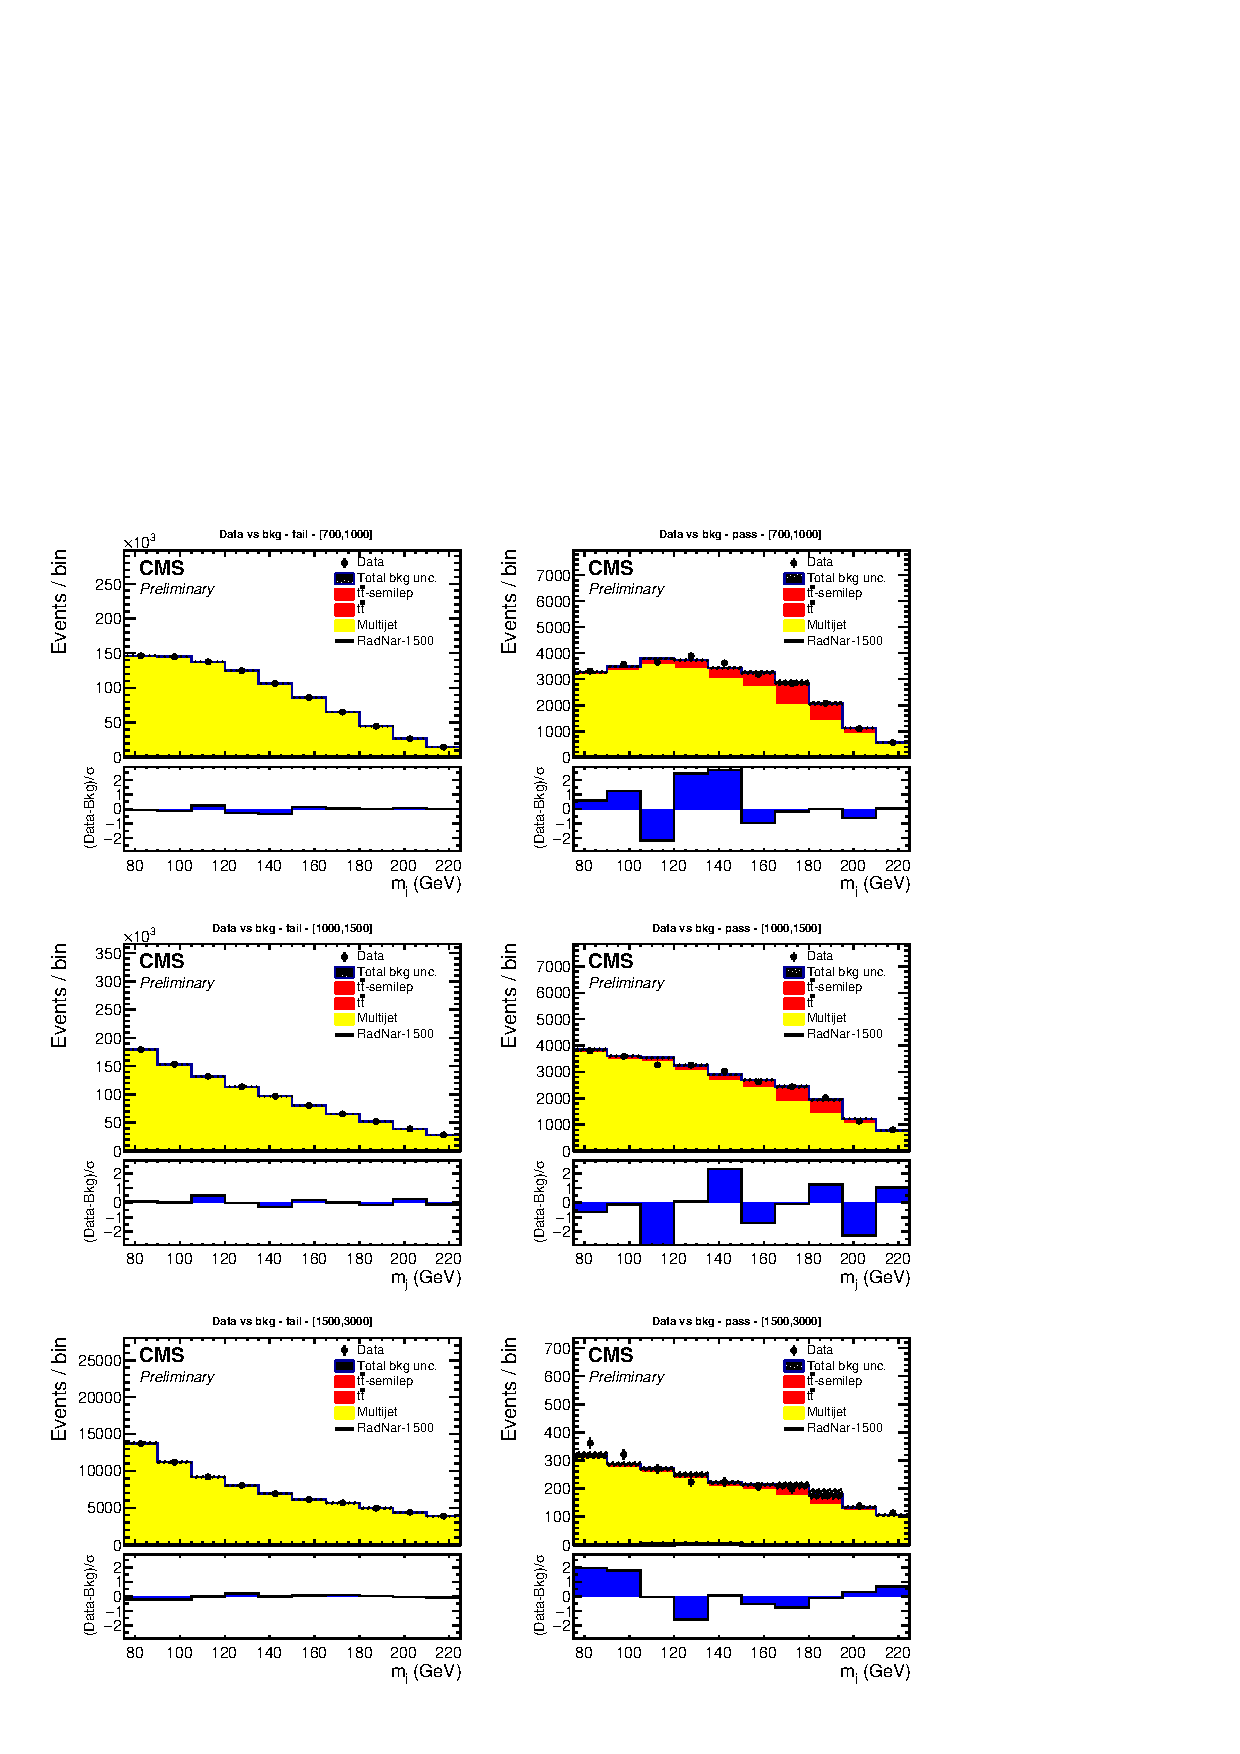
\includegraphics[width=1\textwidth]{Figures/postfit_projx_fitb_CR.pdf}
	\caption{Full Run 2 CR background fits for $M_j$ axis.}
	\label{fig:18CRmj}
\end{figure}
\begin{figure}[!htb]
	\centering
	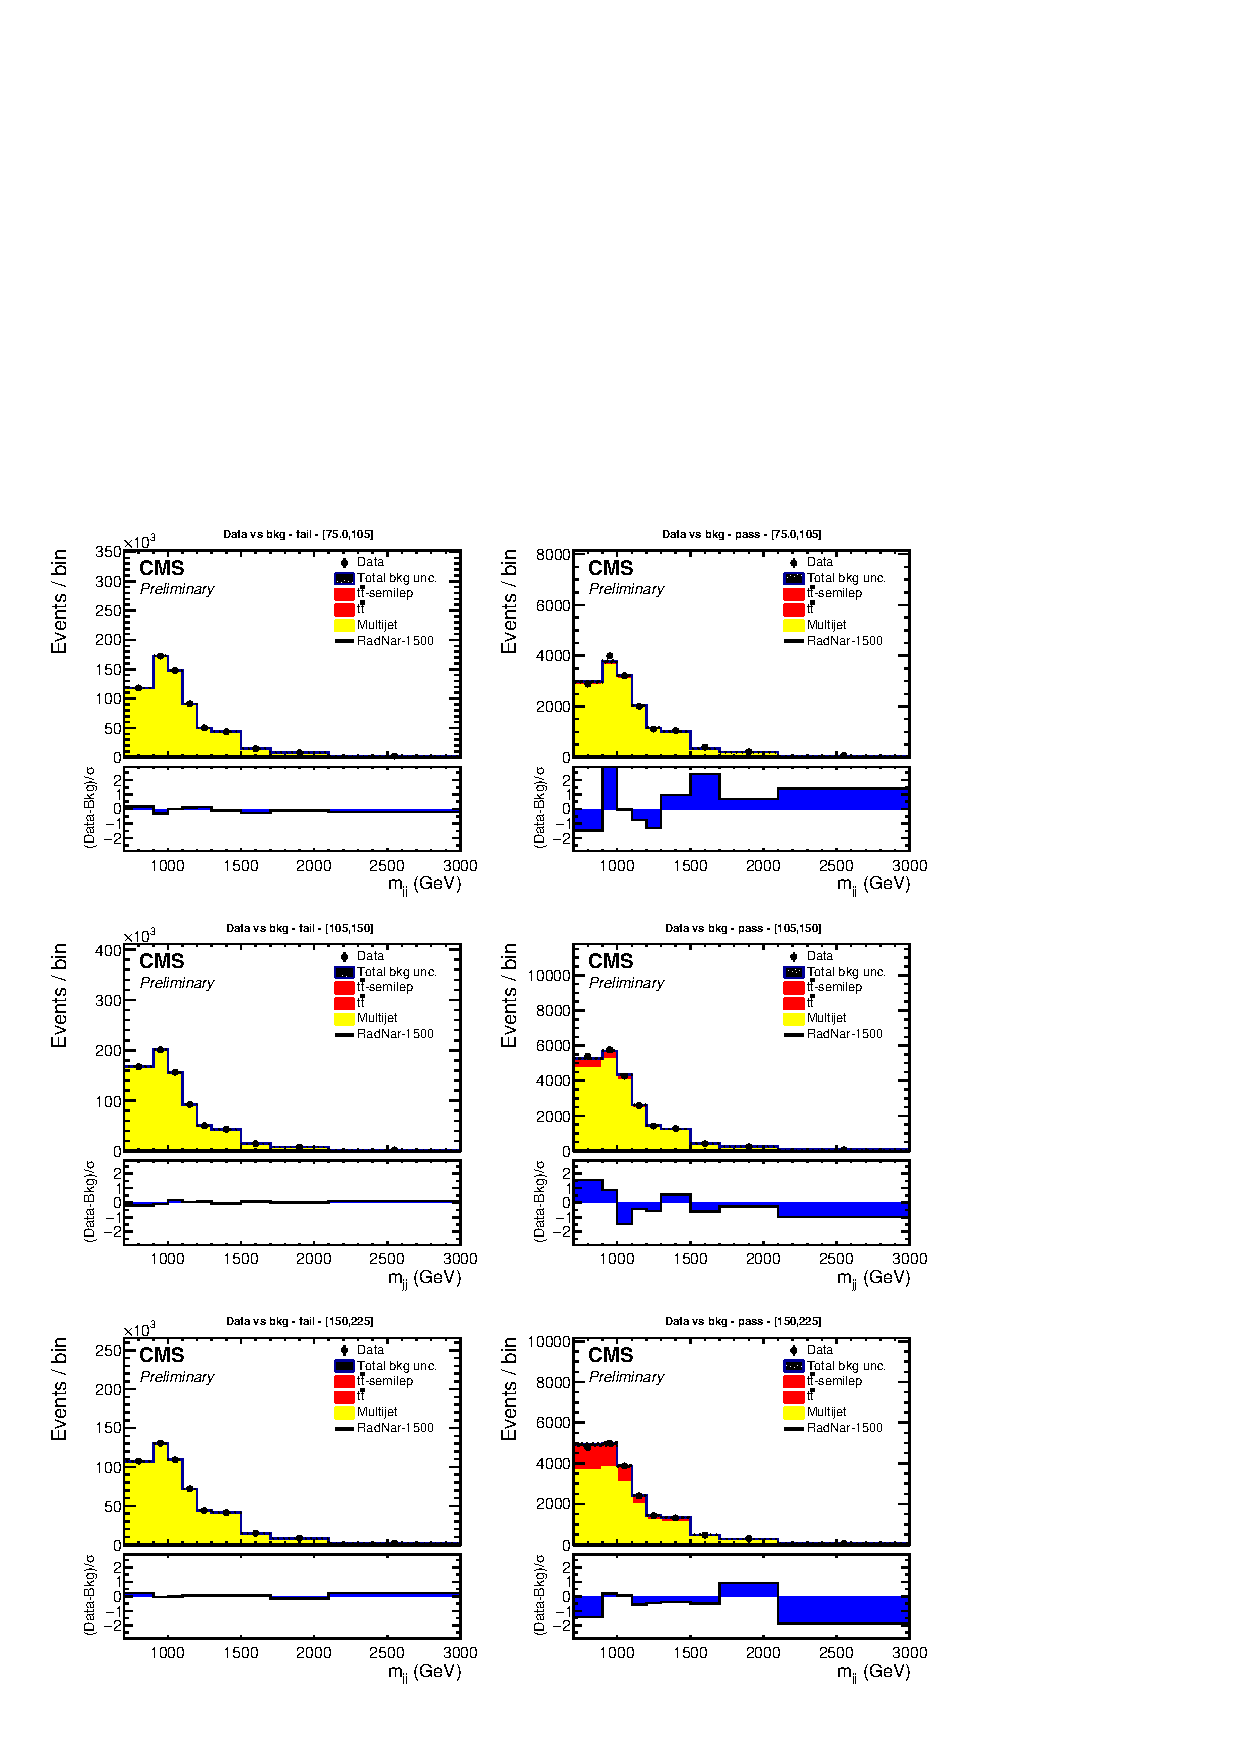
\includegraphics[width=1\textwidth]{Figures/postfit_projy_fitb_CR.pdf}
	\caption{Full Run 2 CR background fits for $M_{jj}$ axis.}
	\label{fig:18CRmjj}
\end{figure}

\clearpage

\subsection{Top Control Region\label{ss:ttbarCR}}
We define a $\ttbar$ control region in order to help constrain the fit to the $\ttbar$ MC background. The event selection is the same as the fully merged topology expect we change the soft drop mass window to be $140 < M_{softdrop} < 210 GeV$ in order to select for the top mass in the subleading H-jet.
\begin{figure}[!htb]
	\centering
	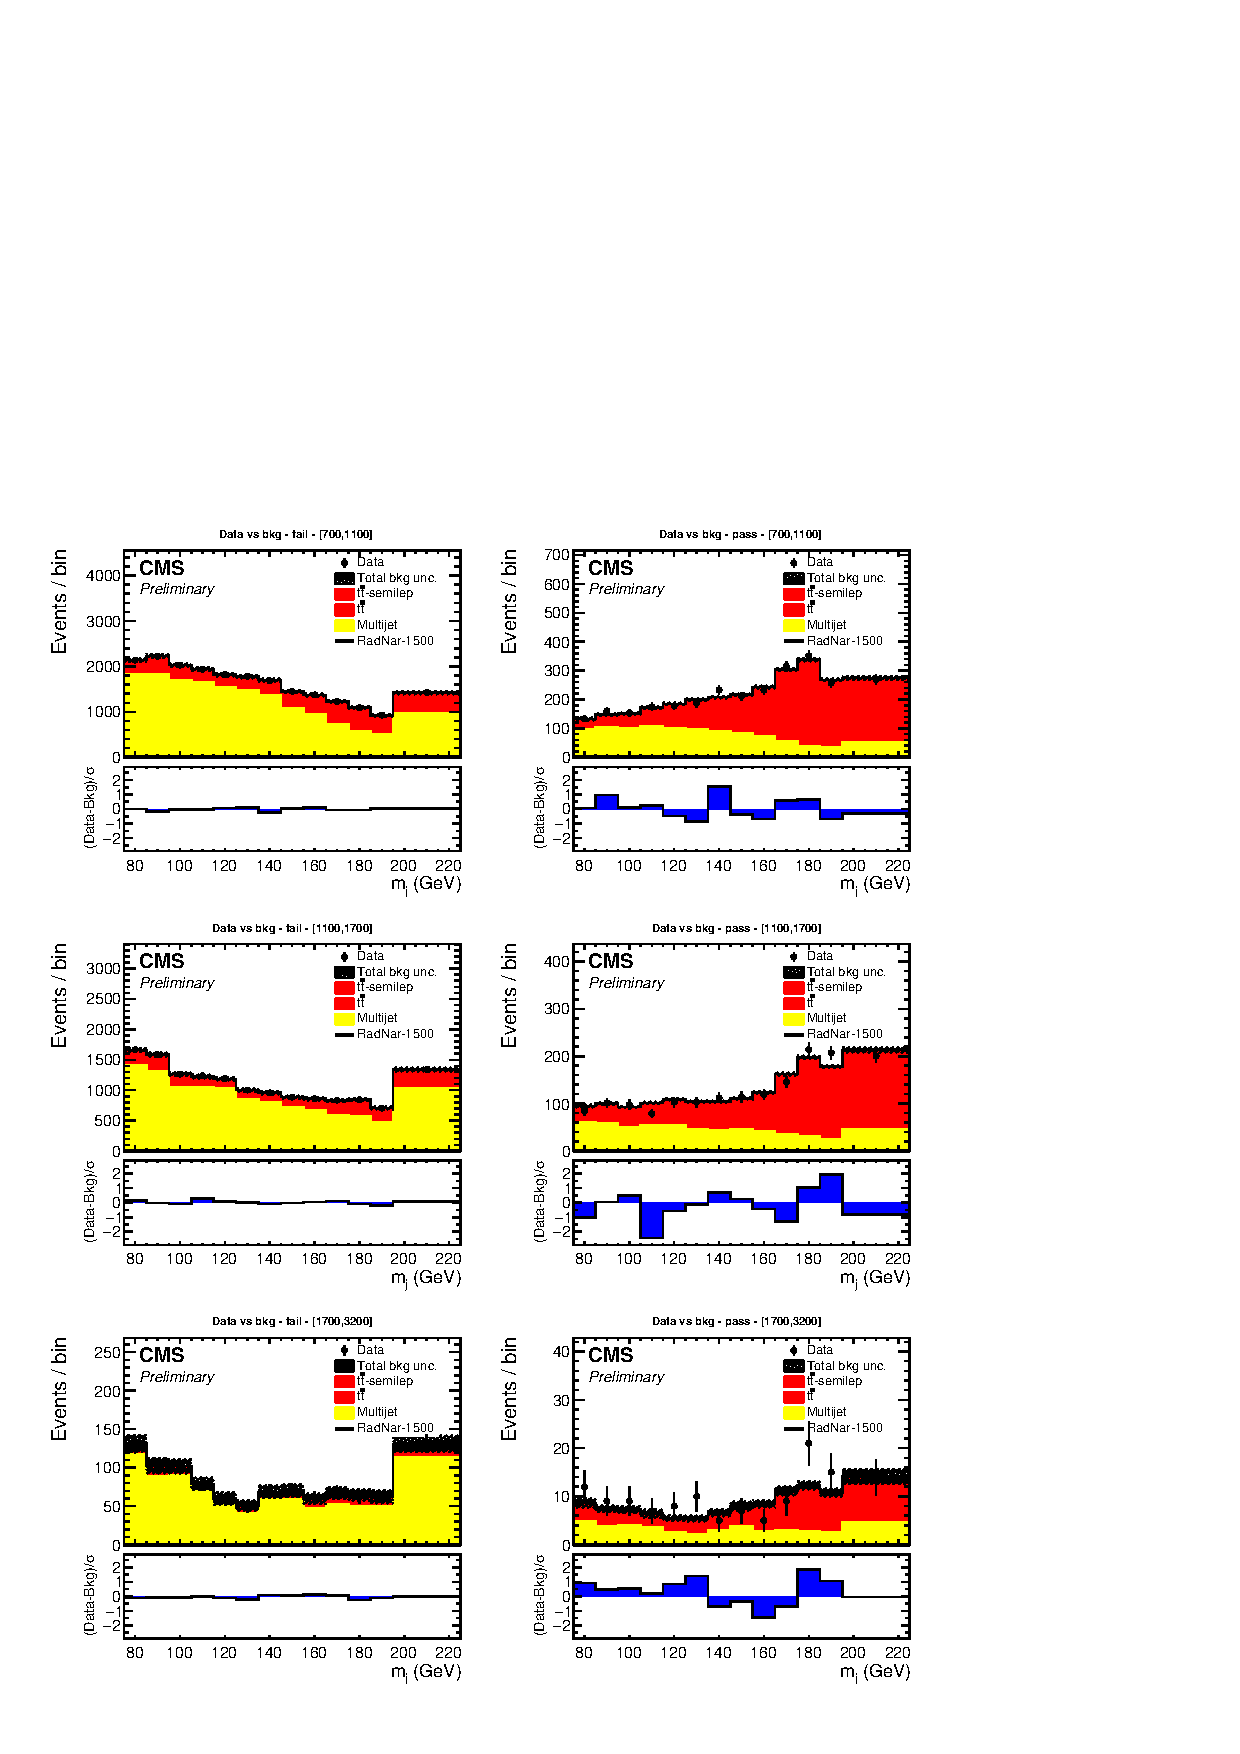
\includegraphics[width=1\textwidth]{Figures/postfit_projx_fits_LLtt.pdf}
	\caption{Full Run 2 Loose Loose $\ttbar$ Control Region fits for $M_j$ axis including expected Radion 1500 GeV signal, normalized to the signal strength found by the fit.}
	\label{fig:LLttmj}
\end{figure}
\begin{figure}[!htb]
	\centering
	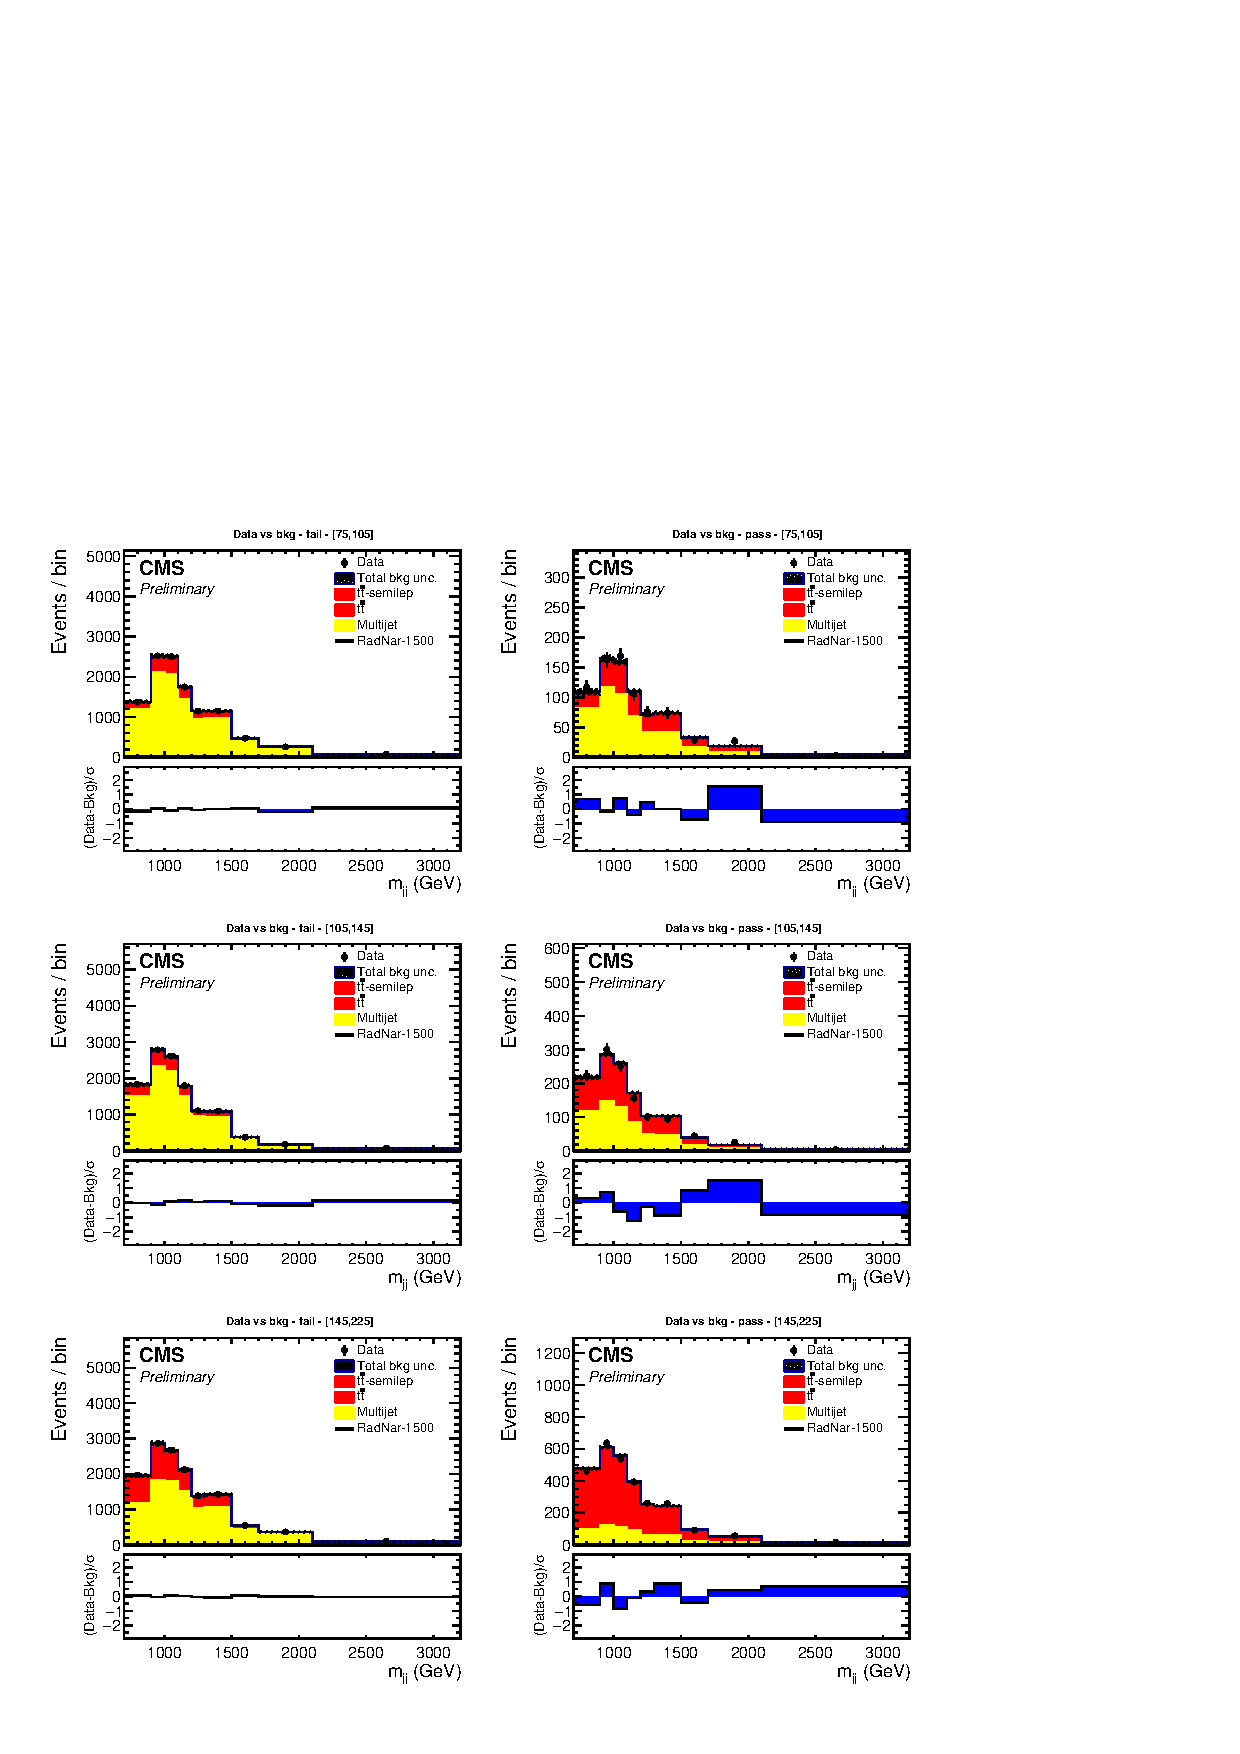
\includegraphics[width=1\textwidth]{Figures/postfit_projy_fits_LLtt.pdf}
	\caption{Full Run 2 Loose Loose $\ttbar$ Control Region fits for $M_{jj}^{red}$ axis including expected Radion 1500 GeV signal, normalized to the signal strength found by the fit.}
	\label{fig:LLttmjj}
\end{figure}
\begin{figure}[!htb]
	\centering
	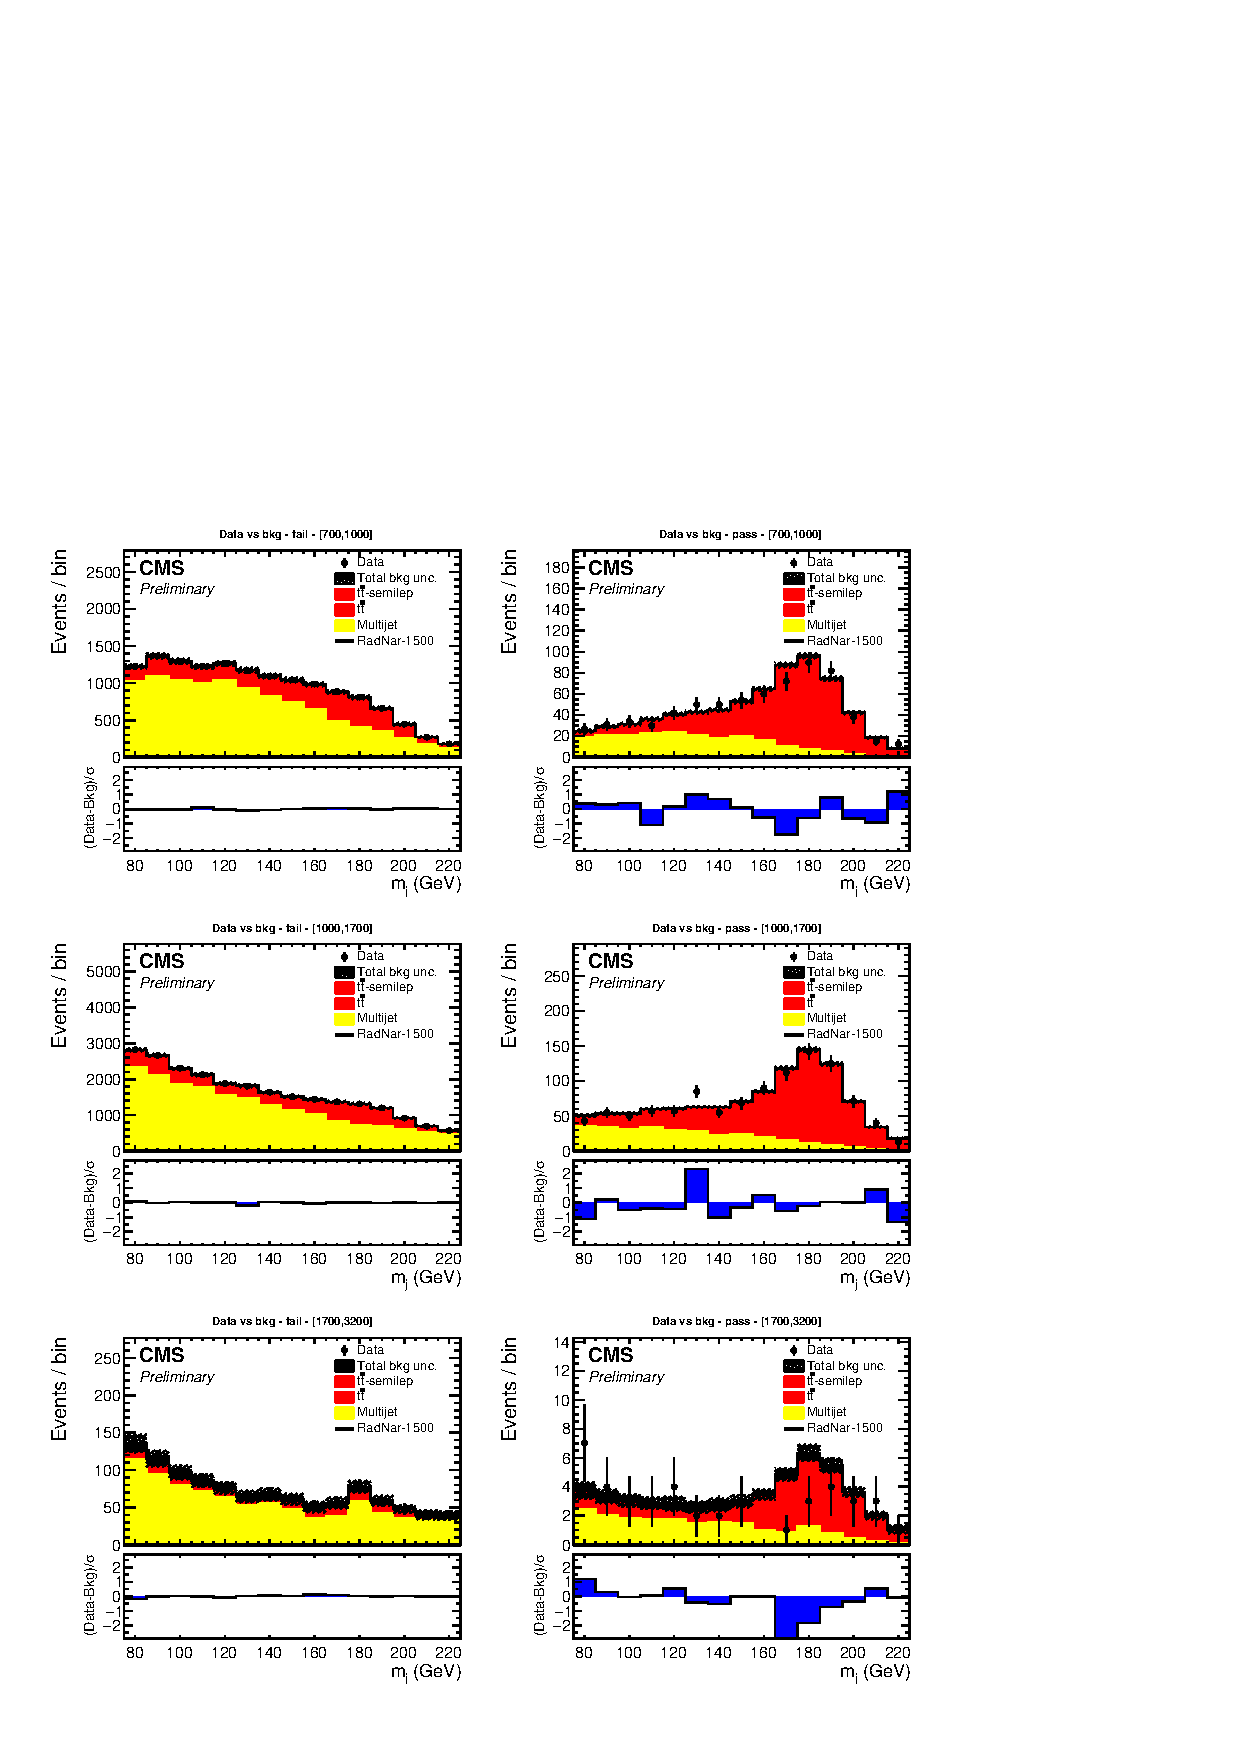
\includegraphics[width=1\textwidth]{Figures/postfit_projx_fits_TTtt.pdf}
	\caption{Full Run 2 Tight Tight $\ttbar$ Control Region fits for $M_j$ axis including expected Radion 1500 GeV signal, normalized to the signal strength found by the fit.}
	\label{fig:TTttmj}
\end{figure}
\begin{figure}[!htb]
	\centering
	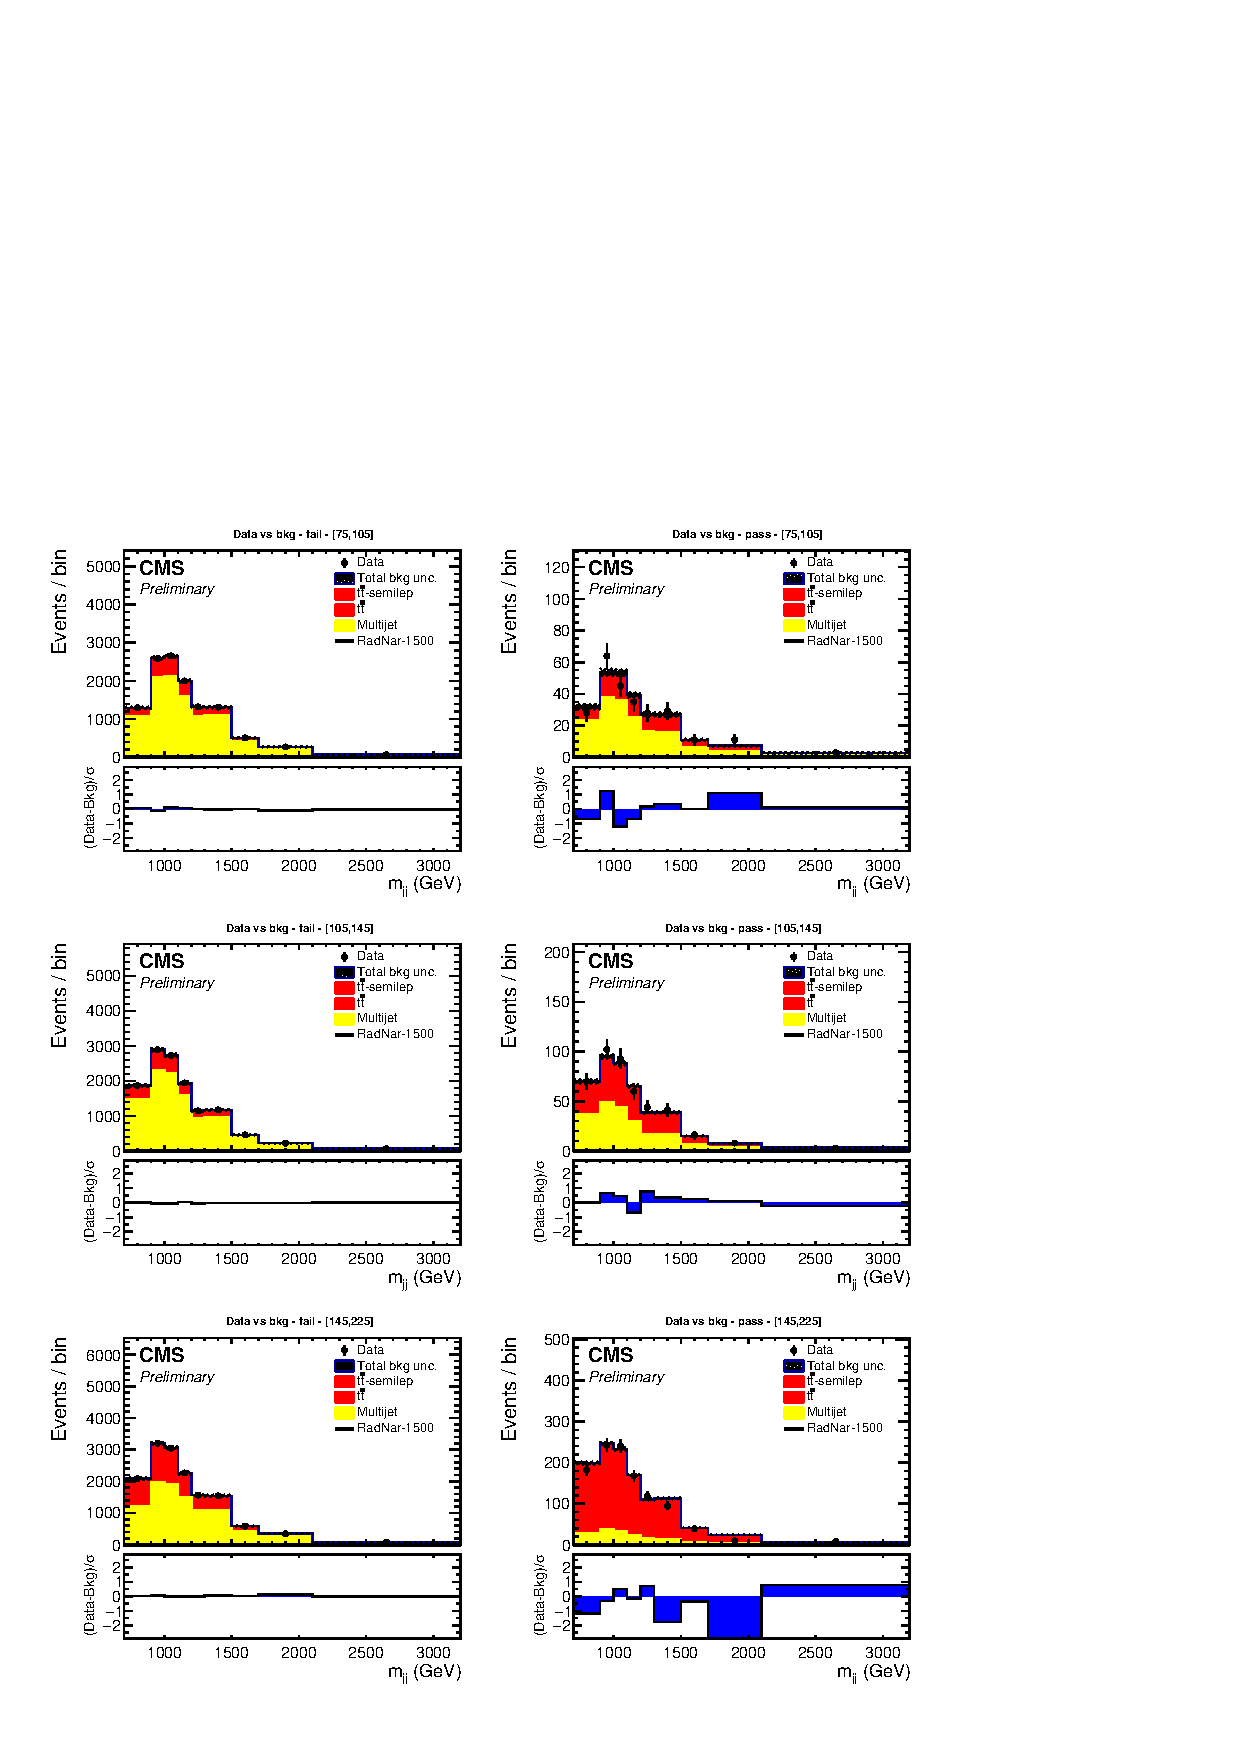
\includegraphics[width=1\textwidth]{Figures/postfit_projy_fits_TTtt.pdf}
	\caption{Full Run 2 Tight Tight $\ttbar$ Control Region fits for $M_{jj}^{red}$ axis including expected Radion 1500 GeV signal, normalized to the signal strength found by the fit.}
	\label{fig:TTttmjj}
\end{figure}
\clearpage
\subsection{Signal Regions Prediction\label{ss:BkgInSigRegion}}
The following section displays the post-fit distributions from the full simultaneous fits performed across the 2016, 2017, and 2018 distributions using the DeepAK8 Mass Decorrelated Hbb tagger.
\begin{figure}[!htb]
	\centering
	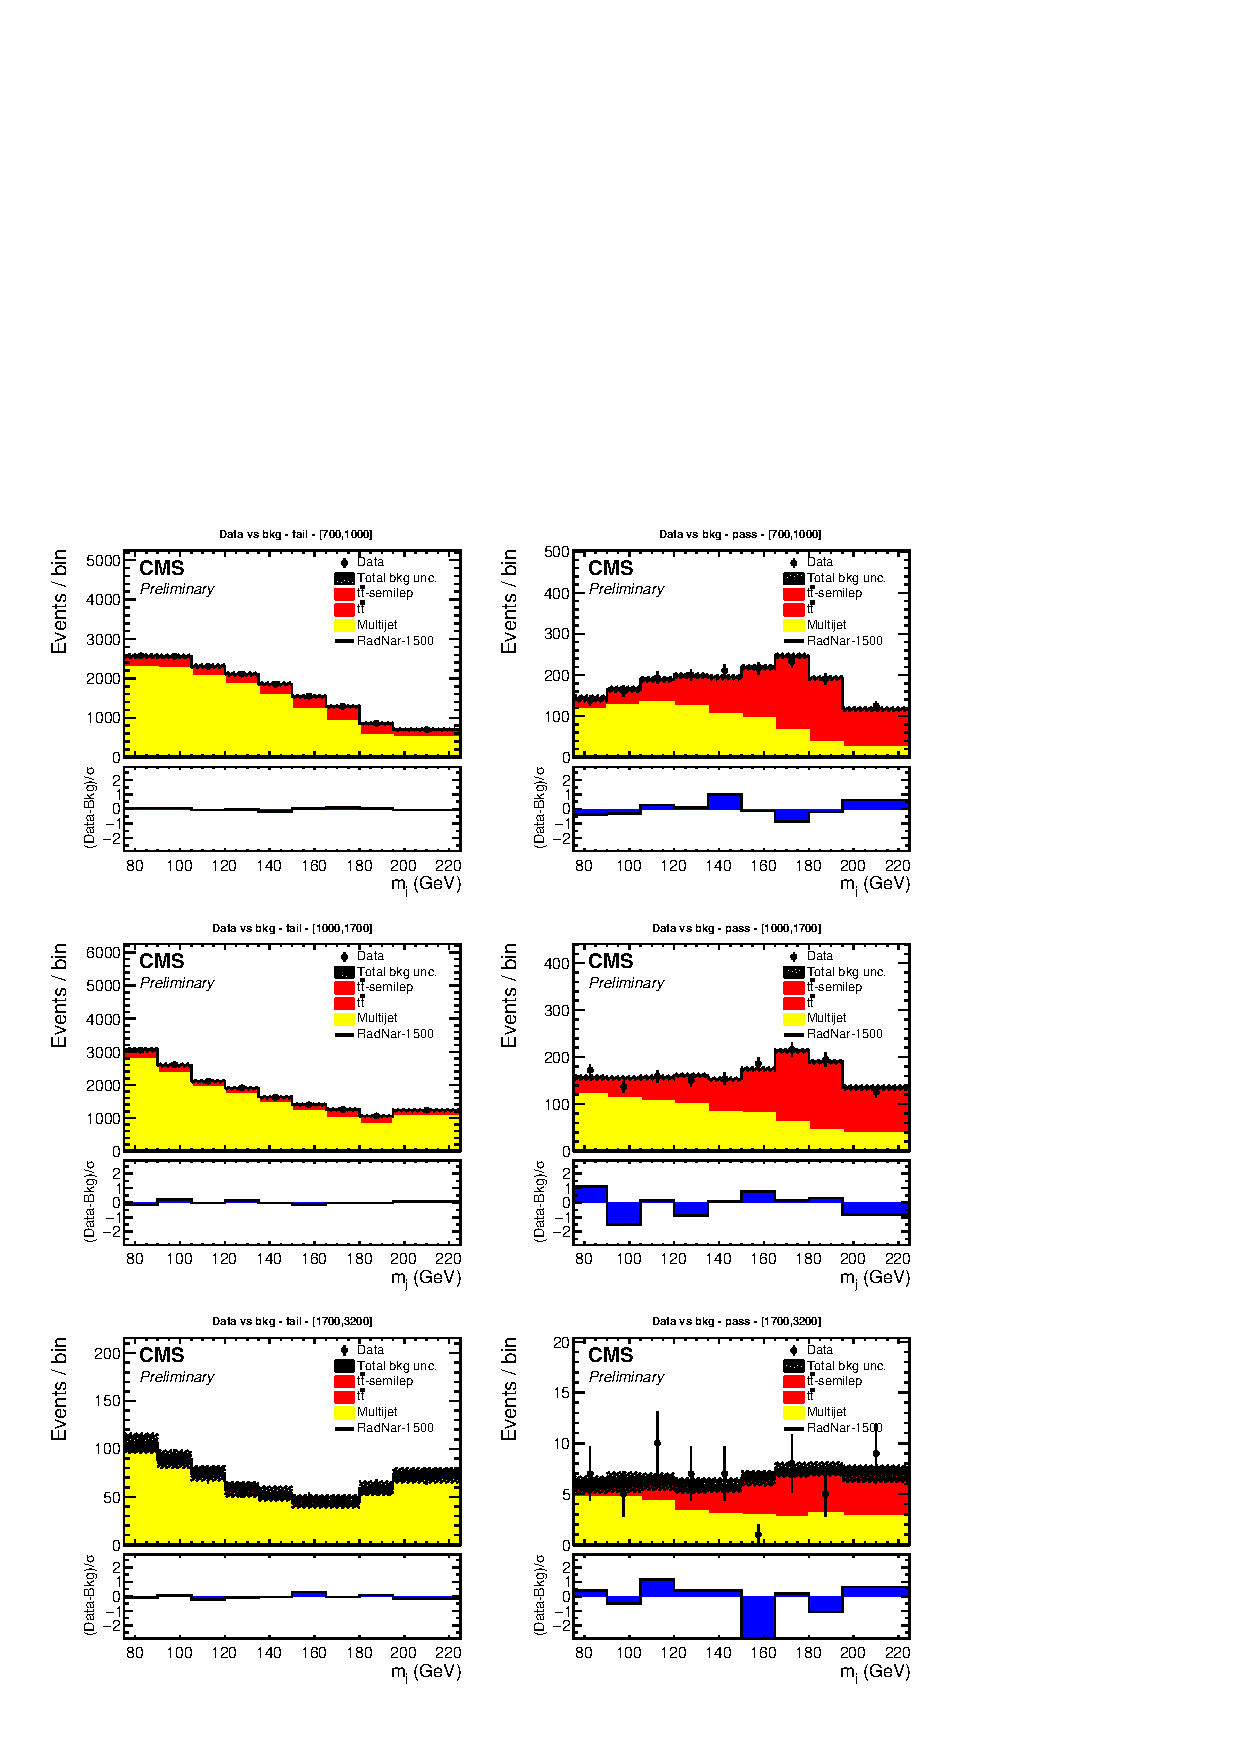
\includegraphics[width=1\textwidth]{Figures/postfit_projx_fits_LL.pdf}
	\caption{Full Run 2 Loose Loose fits for $M_j$ axis including expected Radion 1500 GeV signal, normalized to the signal strength found by the fit.}
	\label{fig:LLmj}
\end{figure}
\begin{figure}[!htb]
	\centering
	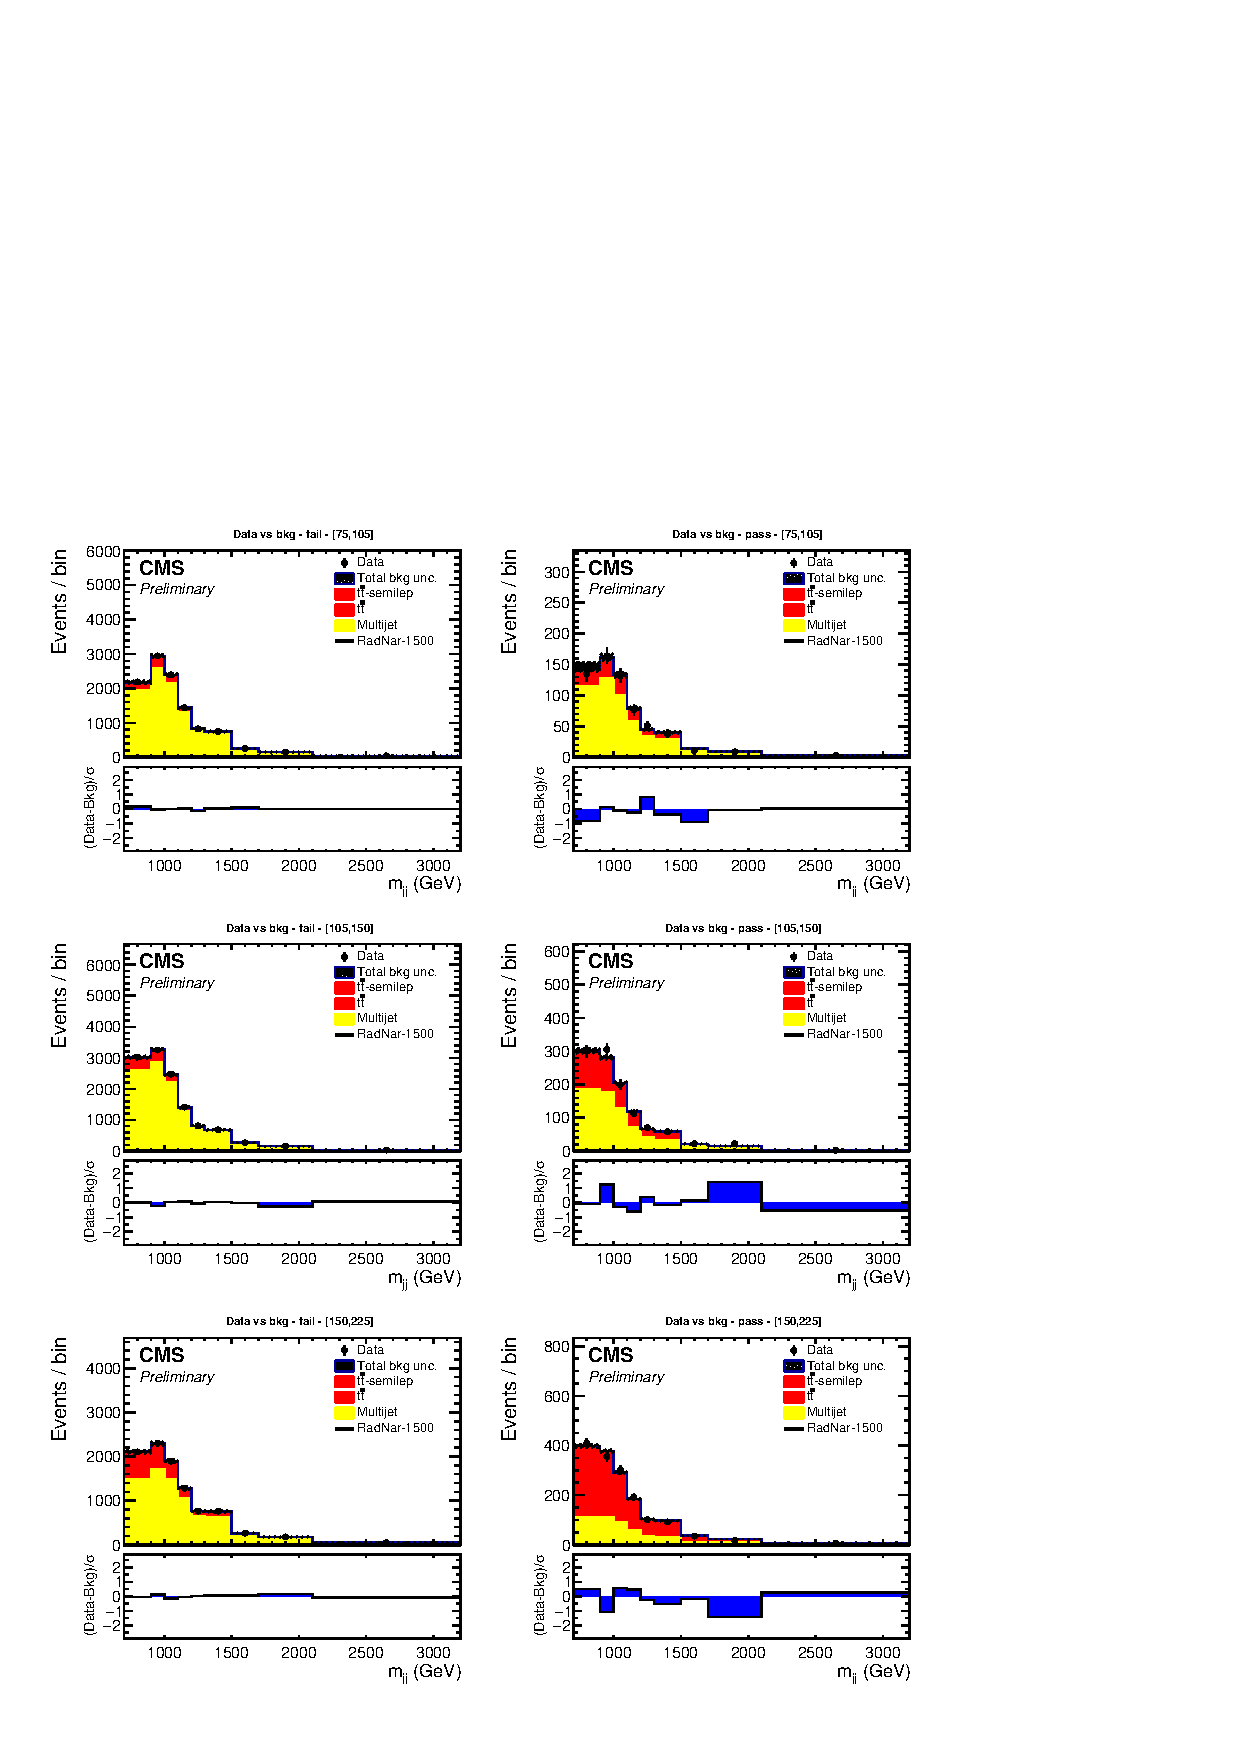
\includegraphics[width=1\textwidth]{Figures/postfit_projy_fits_LL.pdf}
	\caption{Full Run 2 Loose Loose fits for $M_{jj}^{red}$ axis including expected Radion 1500 GeV signal, normalized to the signal strength found by the fit.}
	\label{fig:LLmjj}
\end{figure}
\begin{figure}[!htb]
	\centering
	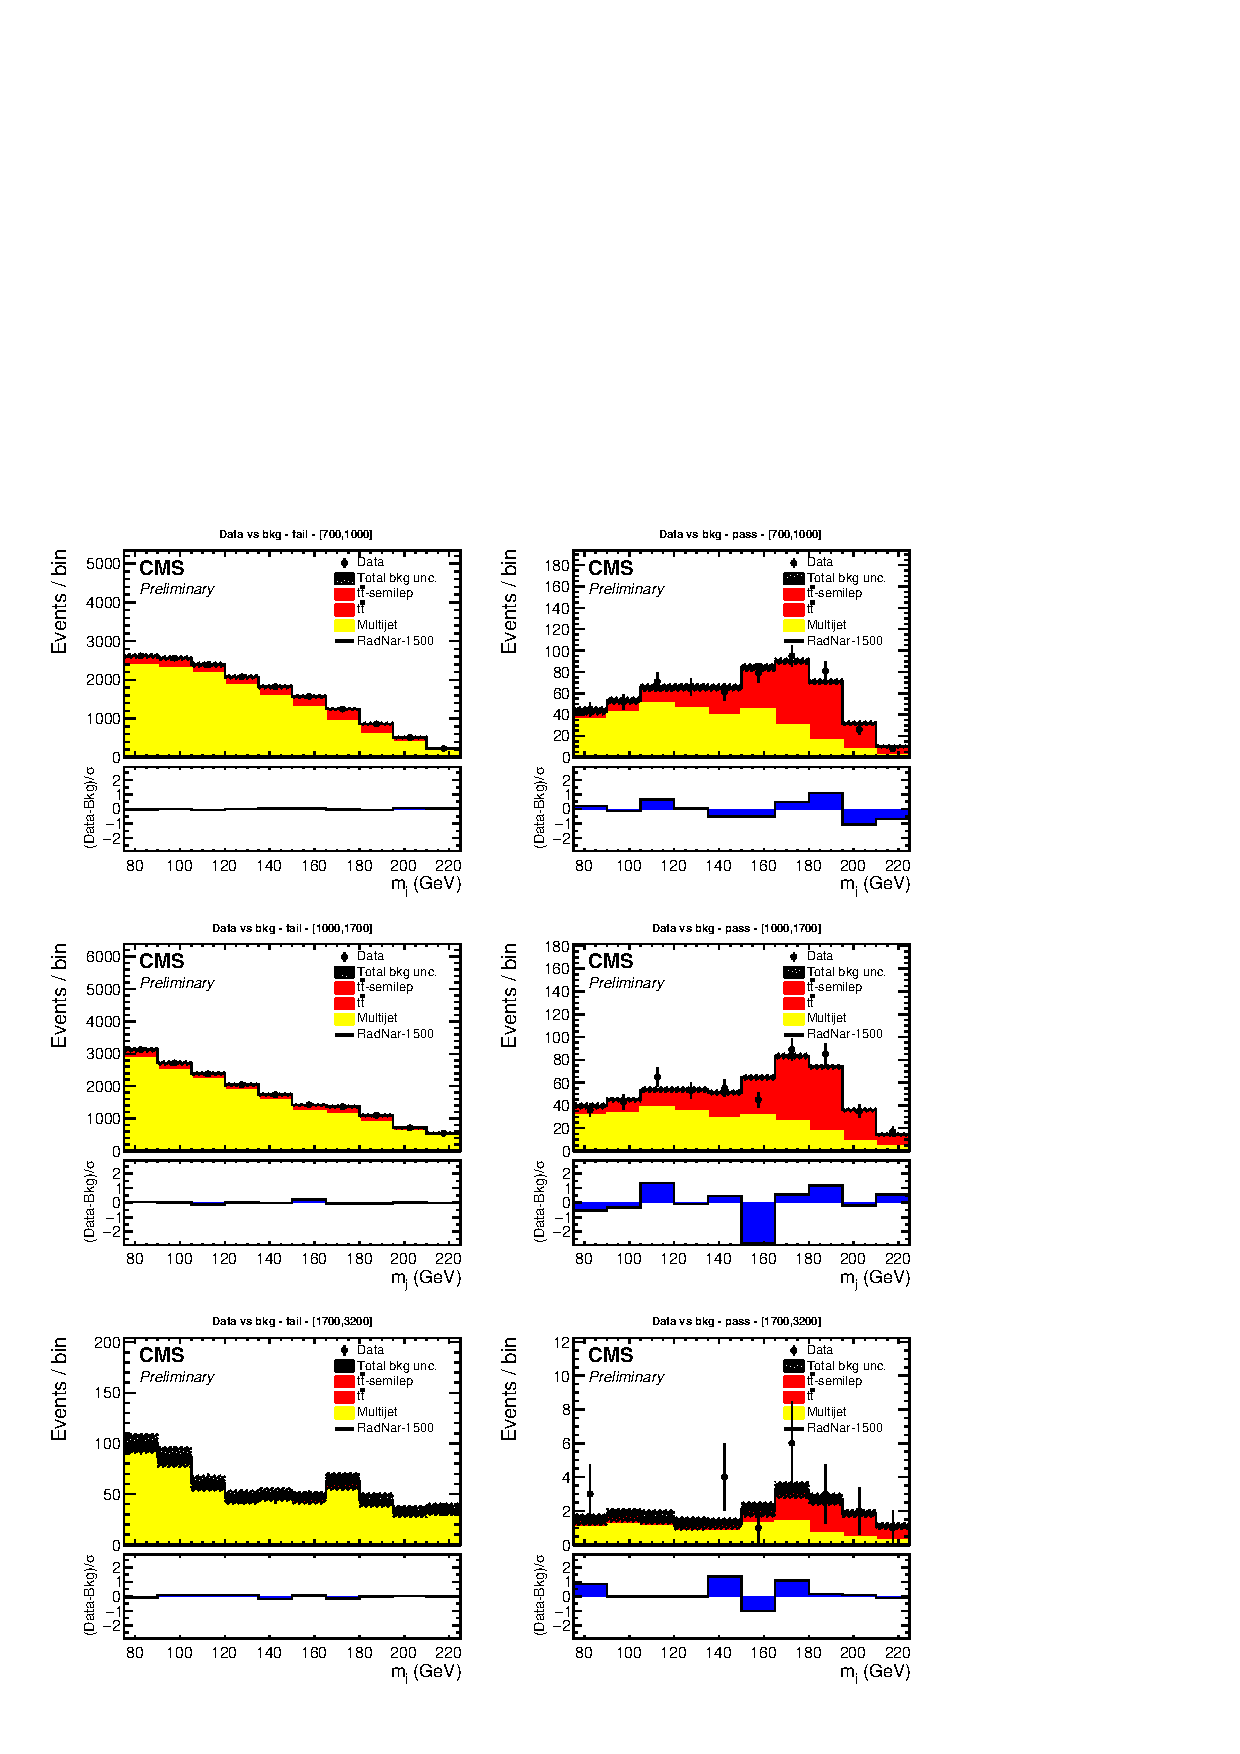
\includegraphics[width=1\textwidth]{Figures/postfit_projx_fits_TT.pdf}
	\caption{Full Run 2 Tight Tight fits for $M_j$ axis including expected Radion 1500 GeV signal, normalized to the signal strength found by the fit.}
	\label{fig:TTmj}
\end{figure}
\begin{figure}[!htb]
	\centering
	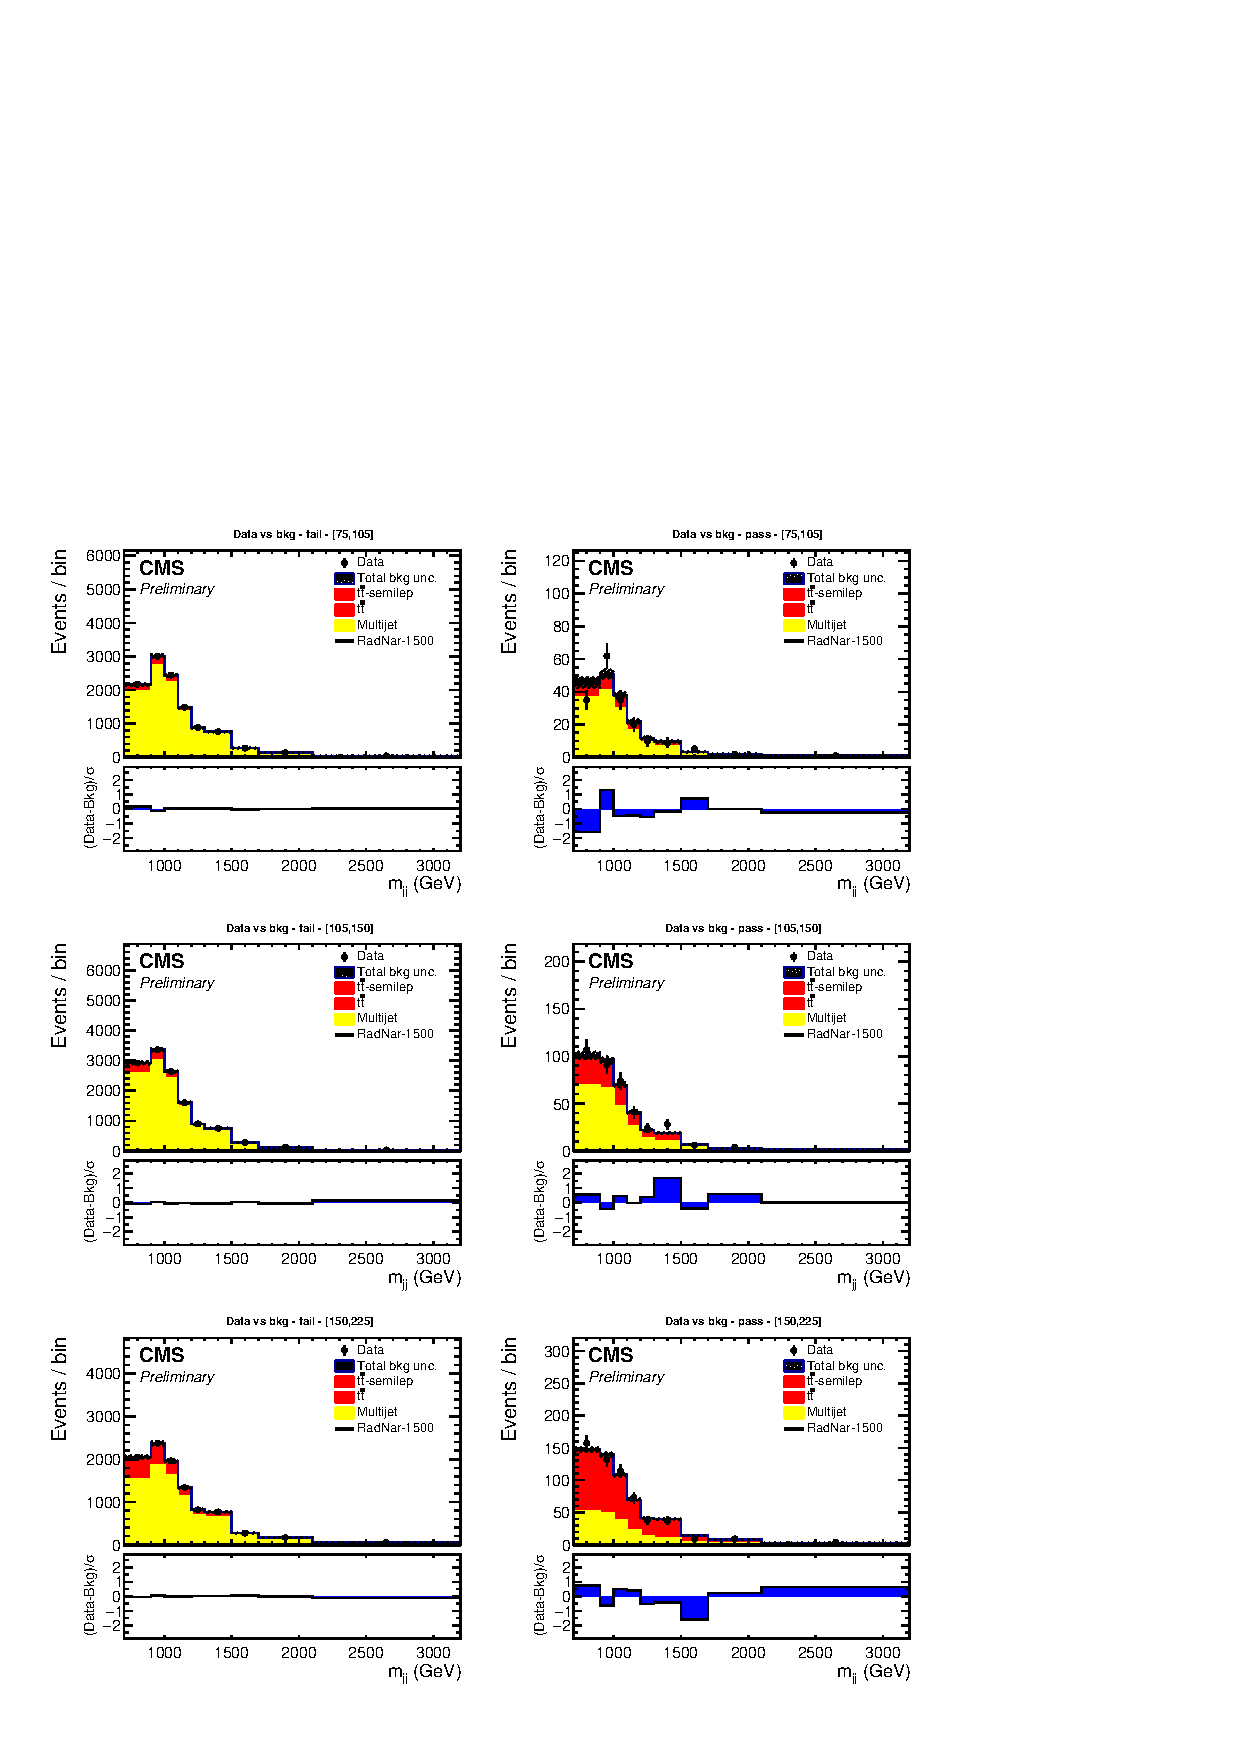
\includegraphics[width=1\textwidth]{Figures/postfit_projy_fits_TT.pdf}
	\caption{Full Run 2 Tight Tight fits for $M_{jj}^{red}$ axis including expected Radion 1500 GeV signal, normalized to the signal strength found by the fit.}
	\label{fig:TTmjj}
\end{figure}
\begin{figure}[!htb]
	\centering
	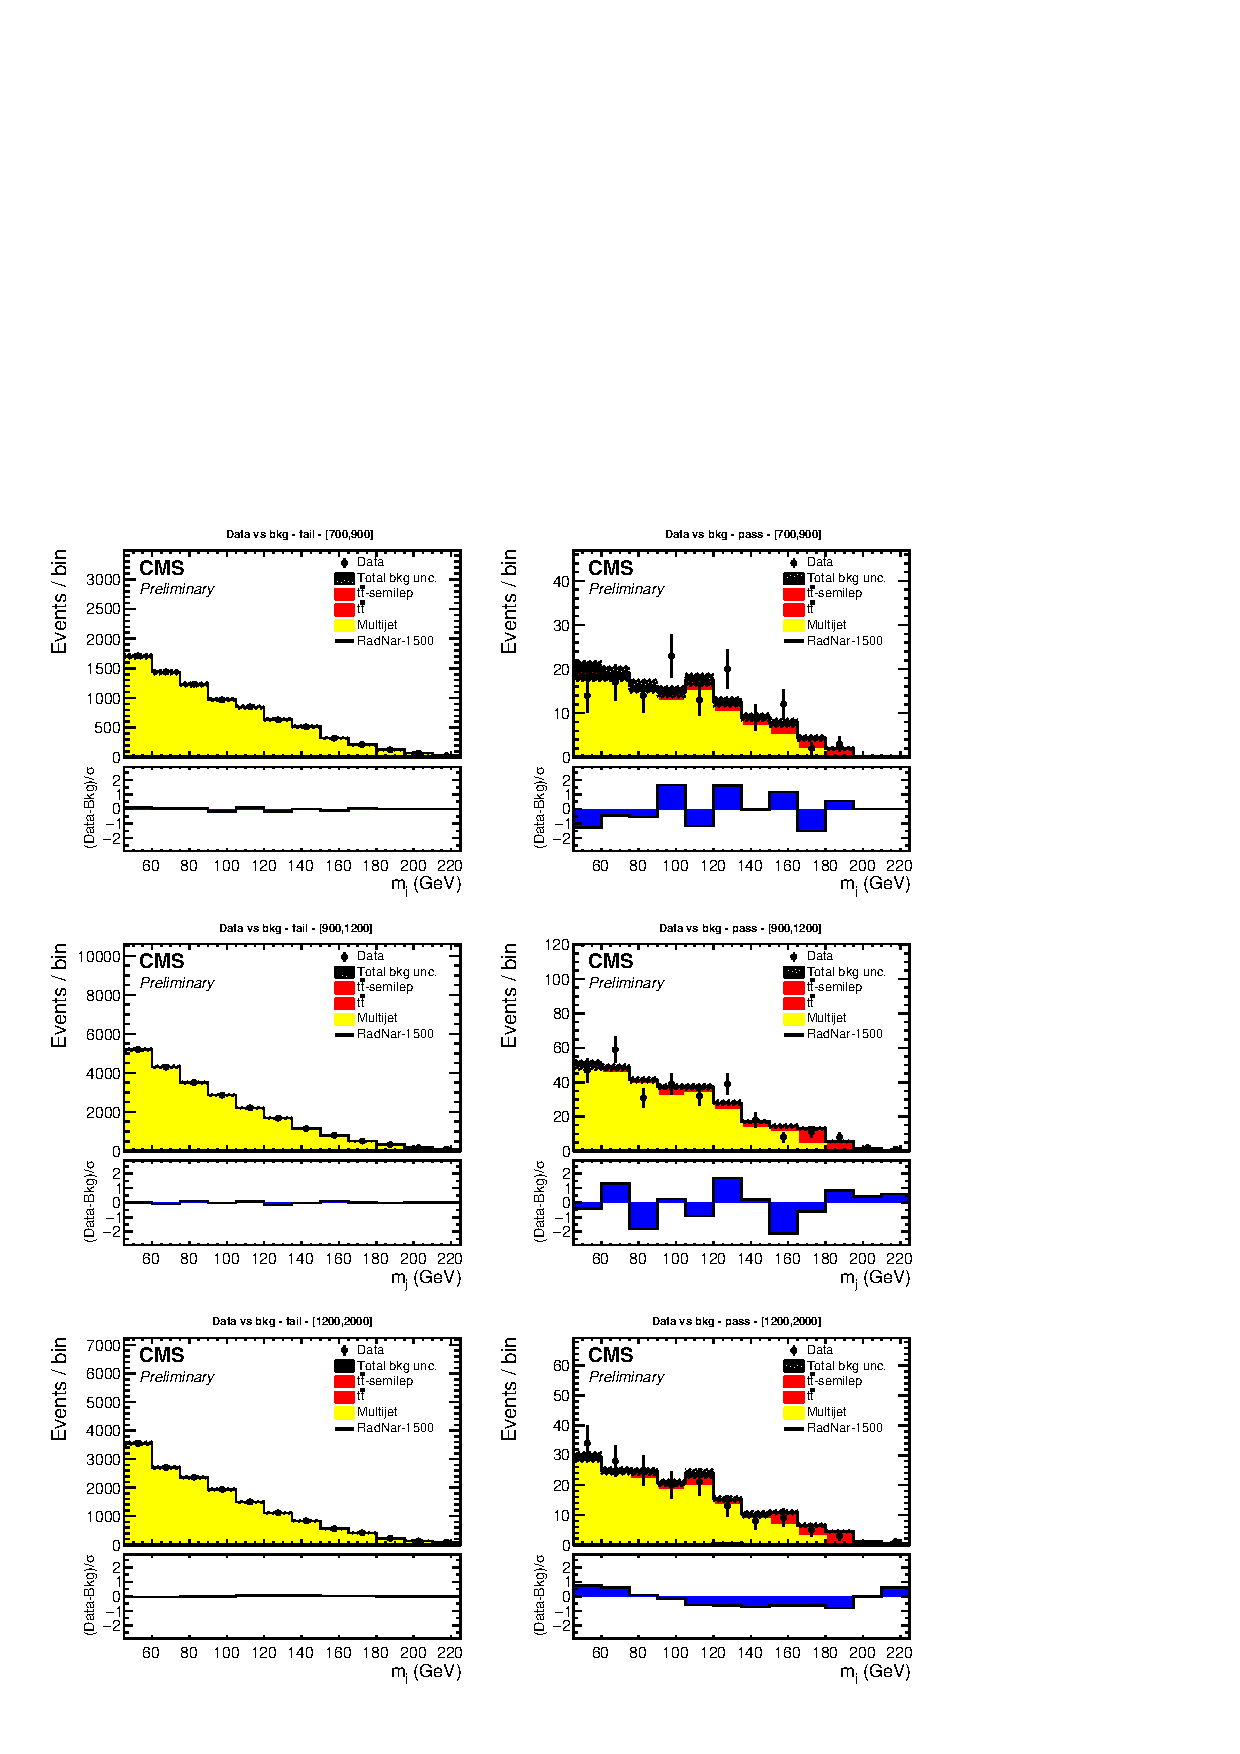
\includegraphics[width=1\textwidth]{Figures/postfit_projx_fits_21.pdf}
	\caption{Full Run 2 2$+$1 fits for $M_j$ axis including expected Radion 1500 GeV signal, normalized to the signal strength found by the fit.}
	\label{fig:21mj}
\end{figure}
\begin{figure}[!htb]
	\centering
	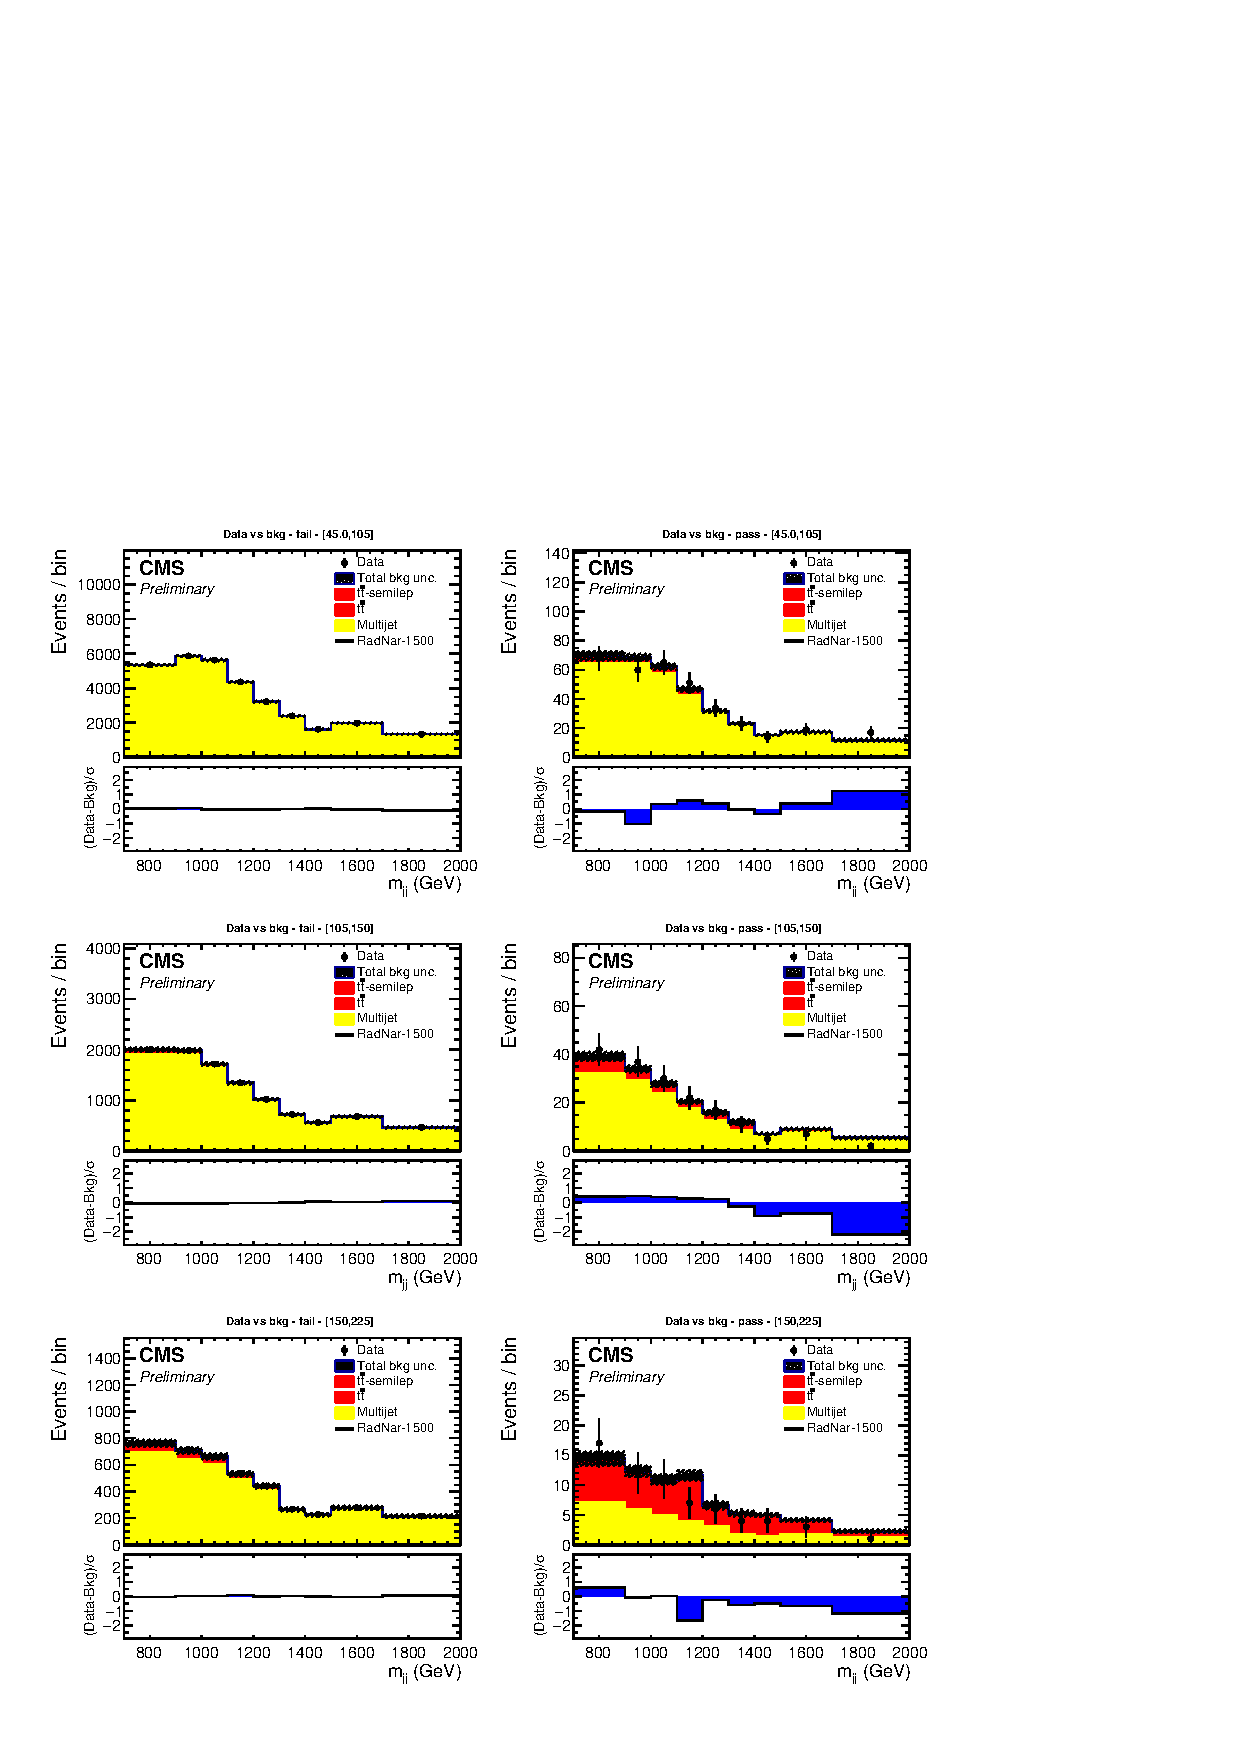
\includegraphics[width=1\textwidth]{Figures/postfit_projy_fits_21.pdf}
	\caption{Full Run 2 2$+$1 fits for $M_{jj}^{red}$ axis including expected Radion 1500 GeV signal, normalized to the signal strength found by the fit.}
	\label{fig:21mjj}
\end{figure}
\begin{figure}[!htb]
	\centering
	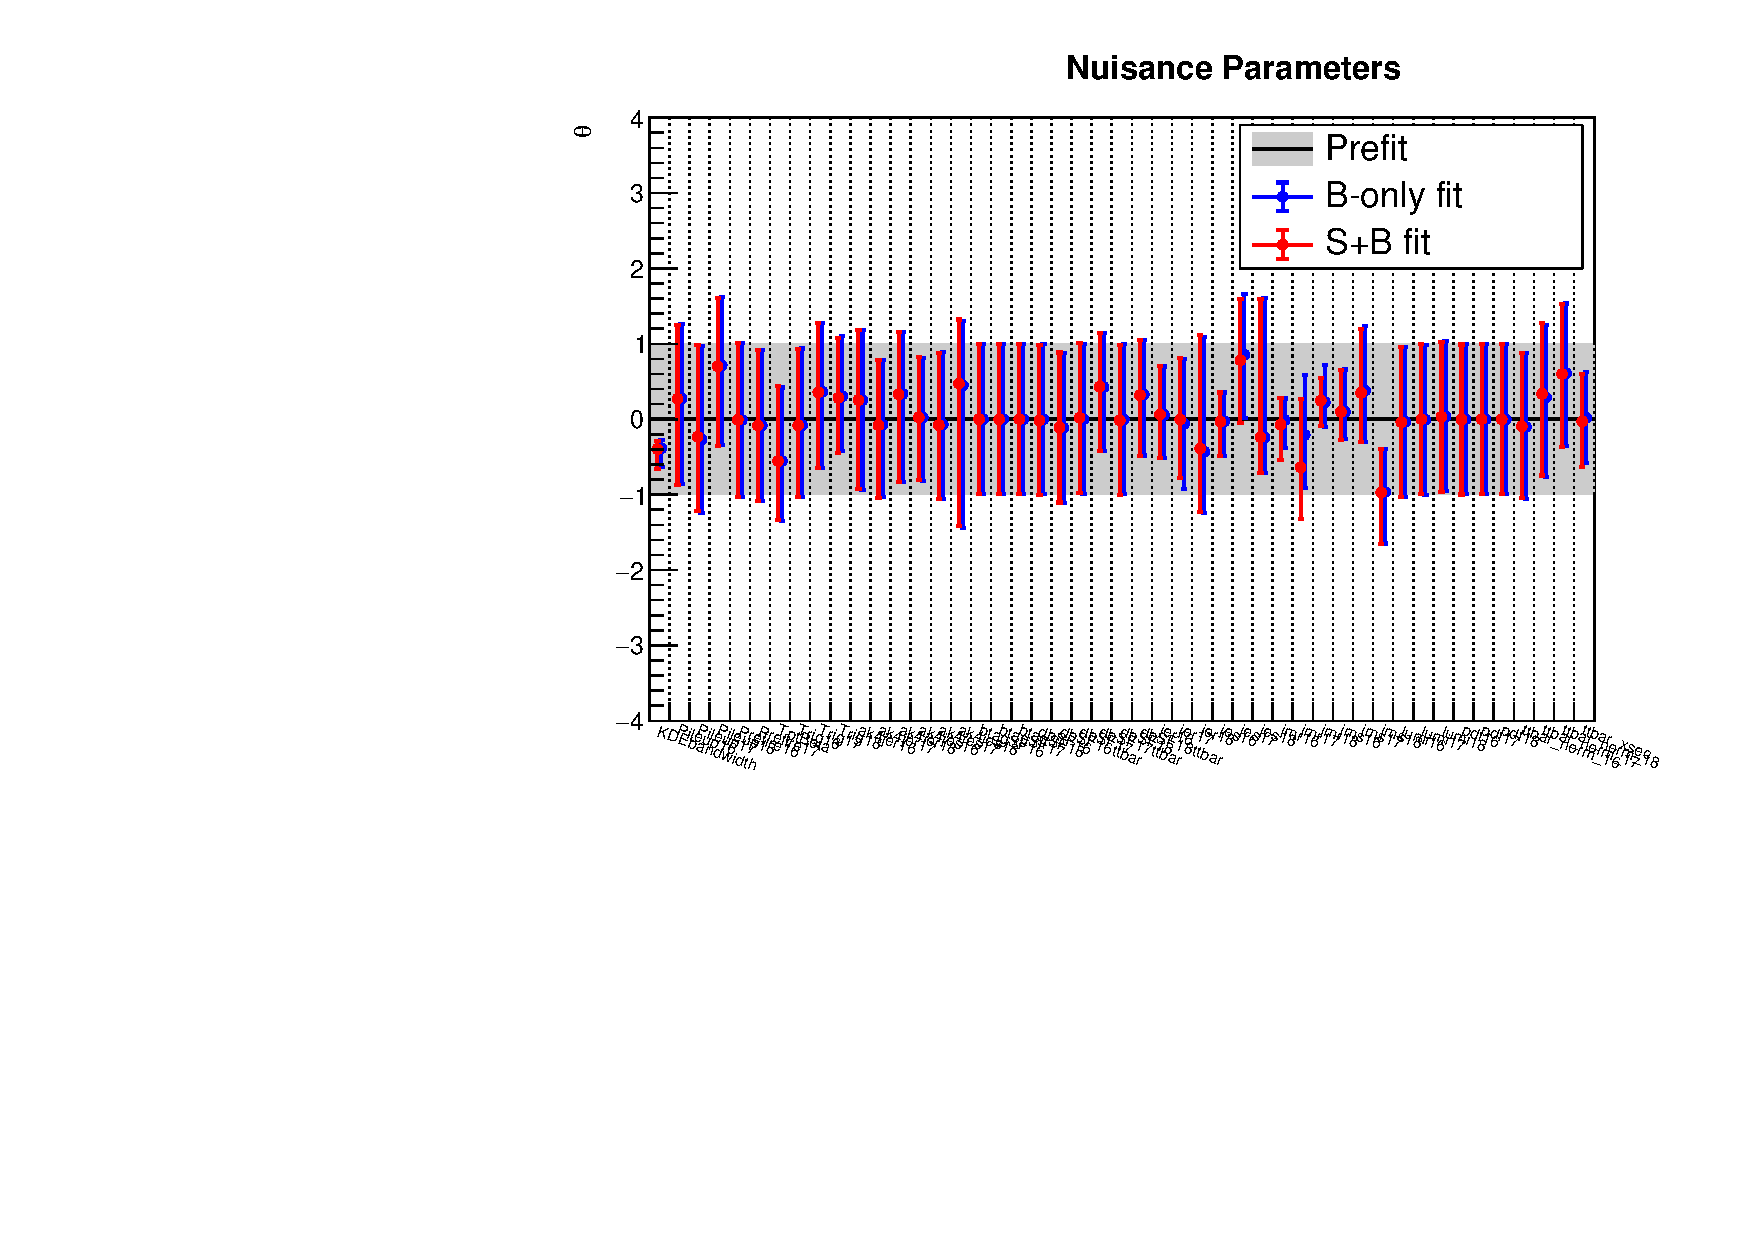
\includegraphics[width=1\textwidth]{Figures/nuisance_pulls.pdf}
	\caption{Full Run 2 Nuisance Pulls Plot.}
	\label{fig:nuissances}
\end{figure}
\begin{figure}[!htb]
	\centering
	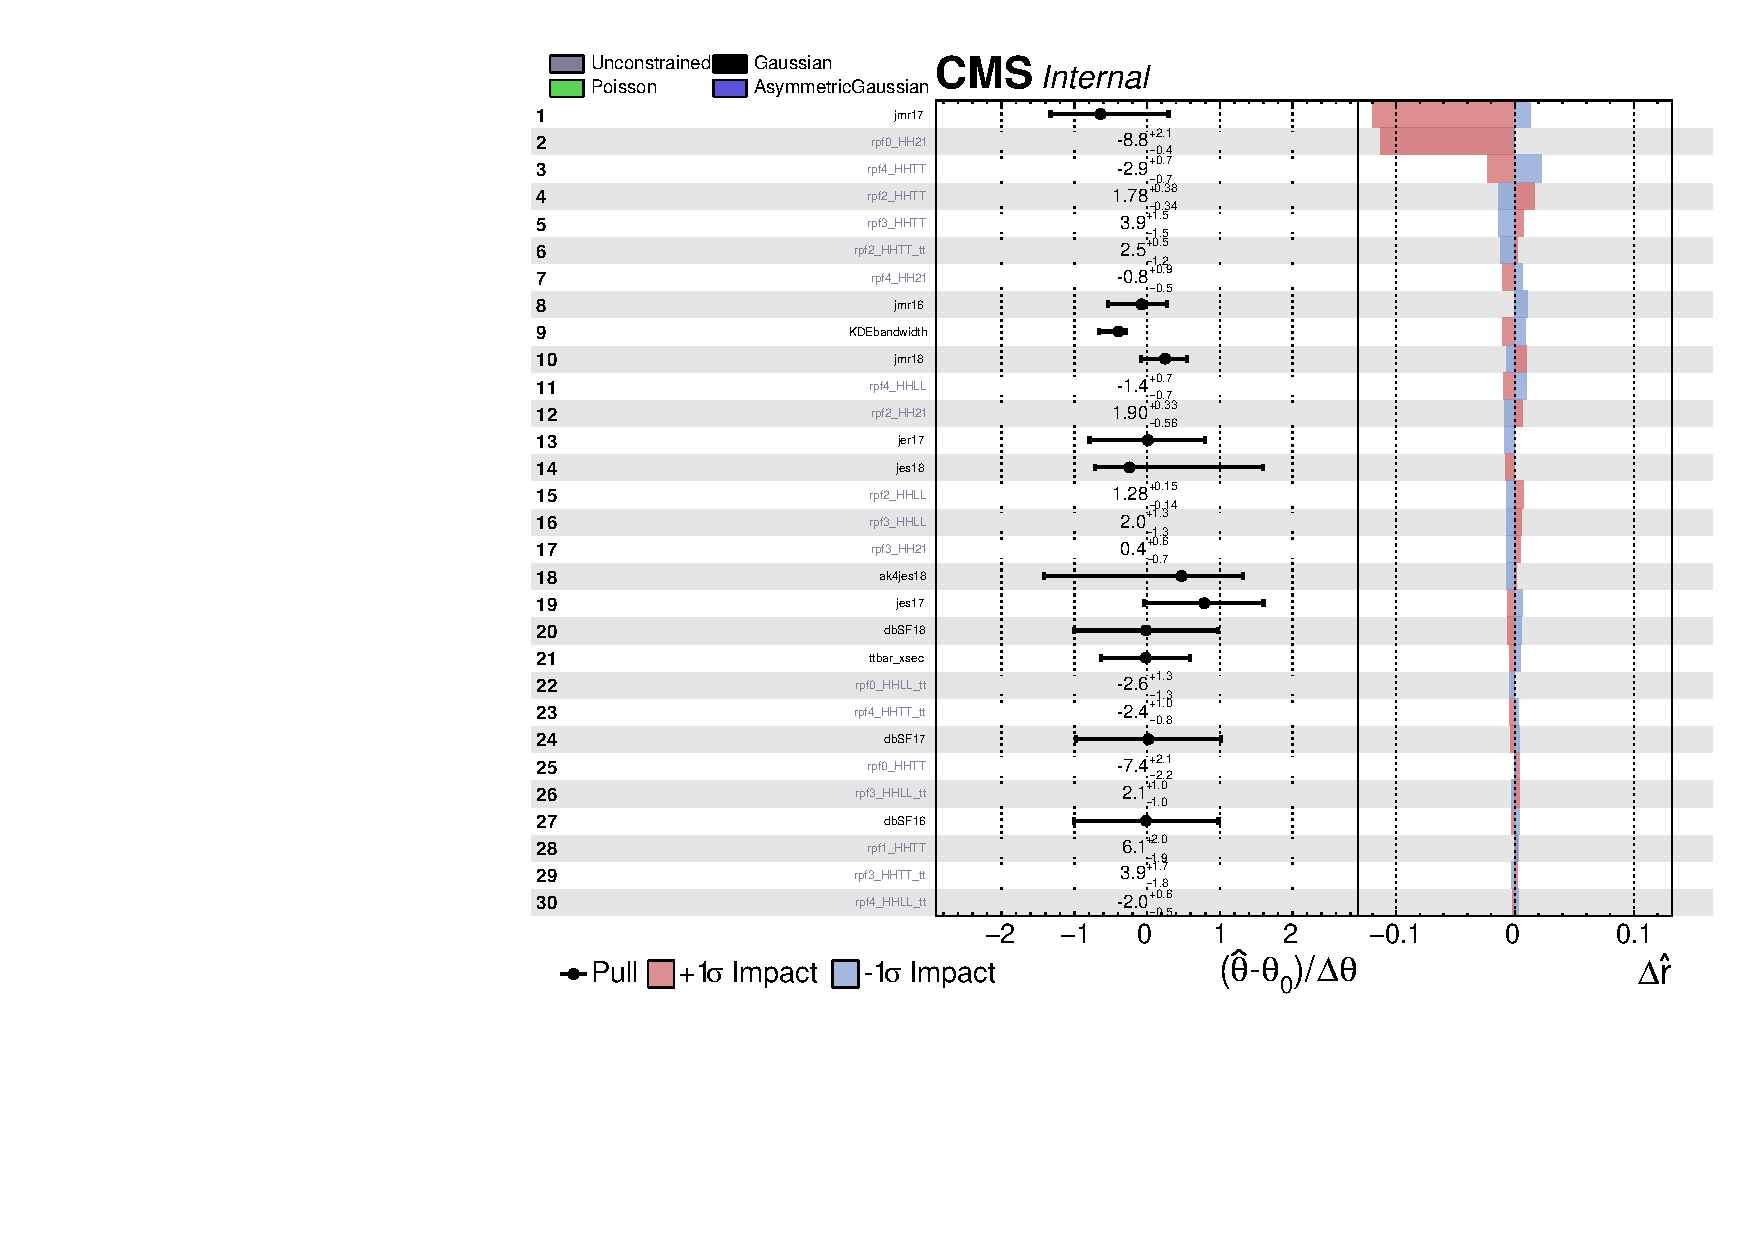
\includegraphics[width=1\textwidth]{Figures/impacts.pdf}
	\caption{Full Run 2 Impacts plot. The impact of a nuisance parameter moving in one direction or another is in some sense a convention. 
	A nuisance parameter that pulls ``negative'' can always be redefined such that the pull will be positive. What one should do is to check to make sure all the nuisance parameters ``pull'' in the correct direction relative to their definition.}
	\label{fig:Impactsplot}
\end{figure}
\clearpage

\section{Systematic Uncertainties\label{sec:Systematics}}

Each of the sources of the systematic uncertainty listed below is represented by at least one nuisance parameter in the fit, controlling either a normalization or a shape of the signal or the $\ttbar$+jets background. The background estimation of QCD is unaffected by them because it is computed entirely from data, which brings with it different procedural sources of systematic uncertainty as described in the following text. We first present the uncertainties that impact the normalization of the signal and $\ttbar$, followed by those which impact the background estimate.

\begin{itemize}

\item \textbf{Luminosity}: An uncertainty of 2.5\%~\cite{CMS-PAS-LUM-17-001} is applied to 2016 and 2018 and 2.3\% is applied to 2017.

\item \textbf{Pileup}: An uncertainty up to 5\% for signal and 1\% for $\ttbar$ is associated with pileup impact on $M_{jj}^{red}$ by varying the estimated minimum bias cross section of pp collisions at 13 TeV (= 69.2 mb) by $\pm 4.6\%$~\cite{PileupTWiki}.

\item \textbf{PDF and scale hypotheses impact}: To estimate the uncertainty from parton distribution functions, we evaluate the RMS of the distribution of the PDF MC replicas. For Hessian sets we compute the square root of the sum of differences squared.Each is used as the $\pm 1 \sigma$ shape variation due to parton distribution functions for their respective sets. Typical uncertainties are $ < 1\% $\\
The PDF set for each sample is as follows:
\begin{itemize}
\item 2016 All Signal Samples: MMHT2015qed\_nlo\_inelastic (MC-Set)
\item 2017 All Signal Samples: NNPDF31\_nnlo\_hessian\_pdfas (Hessian)
\item 2018 All Signal Samples: NNPDF31\_nnlo\_hessian\_pdfas (Hessian)
\end{itemize}


\item \textbf{$\ttbar$ Cross Section Uncertainty}: The total uncertainty, calculated as the sum in quadrature of the scale uncertainty and the PDF+$\alpha_S$ uncertainty on the cross section of $\ttbar$ is applied, amounting to 6\%, as prescribed by the TOP PAG group: $\sigma_{t \bar t}$ = = 831.76 +19.77-29.20 (scale) +35.06-35.06 (PDF+alpha s) pb. 

\item \textbf{Trigger efficiency uncertainty}: The trigger strategy is described in Section~\ref{s:trigger}. The uncertainty of the scale factor is treated as a shape based uncertainty and the template shapes are derived using the maximum of either $\Delta TriggerEff  = 0.05*(1.0-jetTriggerWeight)$ or the Clopper-Pearson error derived from the trigger efficiency for each jet to calculate the $\pm 1 \sigma$ distributions.
  
\item \textbf{Top $p_T$ re-weighting}: In order to account for differences between the shapes of the measured and simulated top $p_T$ spectra, due to the absence of NNLO in the simulation, for $\ttbar$ samples \cite{top-pog}, we nominally re-weight our $\ttbar$ MC samples using the TOP group’s $p_T$-dependent scale factor. For a given event, we apply the nominally derived weight as:
\begin{equation}
SF(p_t) = e^{(\alpha-\beta p_T)}
\end{equation}
and the nominal weight is given as: $W = \sqrt{SF(t)SF(\bar{t})}$ and the nominal parameters are $\alpha = 0.0615$ and $\beta = 0.0005$. Then to create the 1$\sigma$ up and down templates we vary $\alpha$ and $\beta$ up and down independently giving us 4 up and down weights. We use a 1 $\sigma$ upper uncertainty of 2.0 times the nominal weight and a 1 $\sigma$ lower uncertainty bound of 0.5 times the nominal weight when varying $\alpha$ and $\beta$.

% \item \textbf{Double-b-tagging}: Scale factors for the double-b tagger are computed in an enriched gluon splitting to \bbbar data sample. Details on the derivation of this SF are provided in Ref.~\cite{DoubleBSFTWiki}. The corresponding uncertainty is about 3-7\% per event. The mistag SFs are applied to $\ttbar$, corresponding to an uncertainty of 3.6\%. 

% \item \textbf{dak8MDHbb-tagging}: Currently the calculation for the dak8MDHbb SF is ongoing. We have taken their preliminary measurements and applied a value of $1.1$ as the center of a gaussian distribution
% with a $1\sigma$ width of $0.2$, wich accounts most of the numbers derived so far. We plan on updating these numbers when the measurement is finished. 
\item \textbf{dak8MDHbb-tagging}: Scale factors for the dak8MDHbb tagger are computed similarly to the double-b tagger scale factors\footnote{ \url{https://indico.cern.ch/event/853828/contributions/3723593/attachments/1977626/3292045/lg-btv-deepak8v2-sf-20200127.pdf}}. We create a template for each $\pt$ bin range and the values are as follows:
\begin{table}[htb]\footnotesize
  \begin{center}
    \caption{List of Scale Factors for LP [0.80-0.90] values of the Deep AK8 MD Hbb Tagger}
    \begin{tabular}{l|c|c|c}
      \hline
      \hline
      Year & 200-500 & 500-600	& 600-Inf \\
      \hline
      2016 &	1.260 $-$0.118/$+$0.103	 & 1.113 $-$0.102/$+$0.100	& 0.954 $-$0.064/$+$0.063\\
      2017 &	1.364 $-$0.194/$+$0.179	 & 1.114 $-$0.108/$+$0.119	& 1.114 $-$0.055/$+$0.090\\
      2018 &	1.233 $-$0.5543/$+$0.269 &	0.975 $-$0.115/$+$1.025 &	0.979 $-$0.058/$+$0.072\\
      \hline
      \hline  
    \end{tabular}  
    \label{tab:dak8HbbSFsLP}
  \end{center}
\end{table}
\begin{table}[htb]\footnotesize
  \begin{center}
    \caption{List of Scale Factors for HP [0.90-Inf] values of the Deep AK8 MD Hbb Tagger}
    \begin{tabular}{l|c|c|c}
      \hline
      \hline
      Year & 200-500 & 500-600	& 600-Inf \\
      \hline
      2016 &	0.951 $-$0.045/$+$0.047 &	0.974 $-$0.044/$+$0.046 &	1.049 $-$0.051/$+$0.045\\
      2017 &	0.937 $-$0.064/$+$0.114 &	0.922 $-$0.054/$+$0.060 &	0.914 $-$0.089/$+$0.091\\
      2018 &	0.966 $-$0.091/$+$0.101 &	0.958 $-$0.065/$+$0.068 &	0.920 $-$0.080/$+0$.089\\
      \hline
      \hline  
    \end{tabular}  
    \label{tab:dak8HbbSFsHP}
  \end{center}
\end{table}
\item \textbf{$\ttbar$-tagging}
The $\ttbar$ deepAK8 tagger scale factor has been split into SF and normalization and both are applied to the $\ttbar$ distributions. The DeepAK8-MD (bb) mis-tagging scale factors (SF) for top events are derived in a single-muon sample dominated by $\ttbar$ events. See section \ref{ss:ttbarSF} for details. 

\begin{table}[htb]\footnotesize
  \begin{center}
    \caption{List of $\ttbar$ Scale Factors for the Deep AK8 MD Hbb Tagger}
    \begin{tabular}{l|c|c|c}
      \hline
      \hline
      Year & $\pt$ Range [GeV] & Scale Factor & Normalization \\
      \hline
      2016 & 300 - 600 & $1.039^{+0.061}_{-0.058}$ & $0.72^{+0.05}_{-0.05}$\\
      2016 & 600 - 800 & $1.035^{+0.105}_{-0.098}$ & $0.65^{+0.06}_{-0.06}$\\
      2016 & $>$ 800 & $1.301^{+0.325}_{-0.266}$ & $0.52^{+0.07}_{-0.07}$\\

      2017 & 300 - 600 & $0.91^{+0.05}_{-0.05}$ & $0.85^{+0.06}_{-0.06}$\\
      2017 & 600 - 800 & $0.93^{+0.11}_{-0.09}$ & $0.87^{+0.08}_{-0.08}$\\
      2017 & $>$ 800 & $1.07^{+0.28}_{-0.25}$ & $0.74^{+0.09}_{-0.09}$\\

      2018 & 300 - 600 & $0.89^{+0.04}_{-0.05}$ & $0.83^{+0.06}_{-0.06}$\\
      2018 & 600 - 800 & $0.94^{+0.08}_{-0.08}$ & $0.89^{+0.08}_{-0.08}$\\
      2018 & $>$ 800 & $1.05^{+0.21}_{-0.19}$ & $0.86^{+0.09}_{-0.09}$\\

      \hline
      \hline  
    \end{tabular}  
    \label{tab:dak8HbbSFs}
  \end{center}
\end{table}

\item \textbf{DeepJet b-tagging}: This is treated as a shape based uncertainty where the nominal and $\pm 1 \sigma$ distributions are calculated with the recommended BTagCalibration reader class. \footnote{For 2016:https://twiki.cern.ch/twiki/bin/viewauth/CMS/BtagRecommendation2016Legacy For 2017:https://twiki.cern.ch/twiki/bin/viewauth/CMS/BtagRecommendation94X For 2018:https://twiki.cern.ch/twiki/bin/viewauth/CMS/BtagRecommendation102X }

%%\item \textbf{\nsub scale factor}: The scale factor for $\tau_{21}$ selection is measured using semi-leptonic $\ttbar$ sample that is a generous source of boosted hadronic $\PW$ bosons~\cite{CMS-AN-17-051}. We correct the signal and $\ttbar$ yield by the SF as recommended from the POG~\cite{Wtagging}: SF$(\nsub < 0.55) = 1.03 \pm 0.14$ for each jet. Additional uncertainty due to the difference bewteen Higgs jets and $\PW$ jets are determined as described below. \fixme{Possibly drop this?}
  
% \item \textbf{Higgs Tagging}: The jet mass correction is also evaluated using $\PW$ jets in semileptonic \ttjets events, amounting to $1 \pm 0.0094$. A jet mass resolution scale factor of $1 \pm 0.20$ is also obtained using the above measurement. These are propagated to the Higgs-tagged jets along with the uncertainties, for both signal and $\ttbar$

% The main differences between the Higgs jets and $\PW$ jets are the different mass scales and jet flavour compositions, leading to a different shower profile in the jets. The procedure for measuring the scale factor to account for this for Higgs-tagged signal jets is described in~\cite{CMS-PAS-B2G-16-026}.
% This is not applied to $\ttbar$, since it has hadronically decaying $\PW$. This uncertainty corresponds to .5-8.8\% depending on signal mass.

\item \textbf{Jet Energy Scale}: To estimate the uncertainty in the jet energy scale, we use the $\pm 1 \sigma$ variations on the jet energy scale derived as a shape based uncertainty from jet energy corrections for AK8/AK4 PFPUPPI jets. The variations are $\eta$ and $p_T$ dependent, and result is a scaling of the jet four momentum prior to the analysis selection.

\item \textbf{Jet Energy Resolution}: We apply the approved jet energy resolution correction, which is $\eta$ dependent and is used to correct for differences in $p_T$ resolution between data and Monte Carlo. The recommended $\pm 1 \sigma$ variations are also taken into into account \footnote{https://twiki.cern.ch/twiki/bin/view/CMS/JetResolution and stored in a private github repo here: https://github.com/lcorcodilos/nanoAOD-tools/tree/master where we updated to the latest v7 nanoAOD tools.} to make a shape based uncertainty. 

\item \textbf{Jet Mass Scale}: We use the $\pm 1 \sigma$ variations on the jet mass scale derived as a shape based uncertainty and do not apply the nominal jet mass correction as it is not appropriate for this analysis.

\item \textbf{Jet Mass Resolution}: We use $\pm 1 \sigma$ variations of the jet mass resolution as a shape based uncertainty. We also do not apply the nominal jet mass resolution correction as it is not appropriate. Examples of all JECs can be seen in appendix \textbf{FIXME} %\ref{s:jerExamples}

\item \textbf{Multijets background from the data}: 
The main source of uncertainty for the non-top background is propagated directly from the error of the fit in mass-sidebands from which we have estimated the transfer factor. This uncertainty can be treated as a shape based uncertainty. We must further account for the statistical uncertainty in the anti-tag region which is propagated to the signal region when the estimate is made. 

\item \textbf{KDE Bandwidth}: The bandwidth used for to smooth qcd has an uncertainty that is treated as shape based uncertainty where the $\pm 1 \sigma$ distributions are made from smoothed qcd distributions made with the value $\pm 1$ used as the bandwidth. Figure \ref{fig:KDETT} shows the up,down, and nominal distributions as an example.
%\item \textbf{TriAK4jet Mass Cut}: The systematic for this cut was calculated by comparing the cut efficiency for the Pythia and Herwig Bulk Graviton 1000 GeV samples, documented in \fixme{XXX}, and is equivalent to 0.5\% systematic. 
\begin{figure}[!htb]
	\centering
  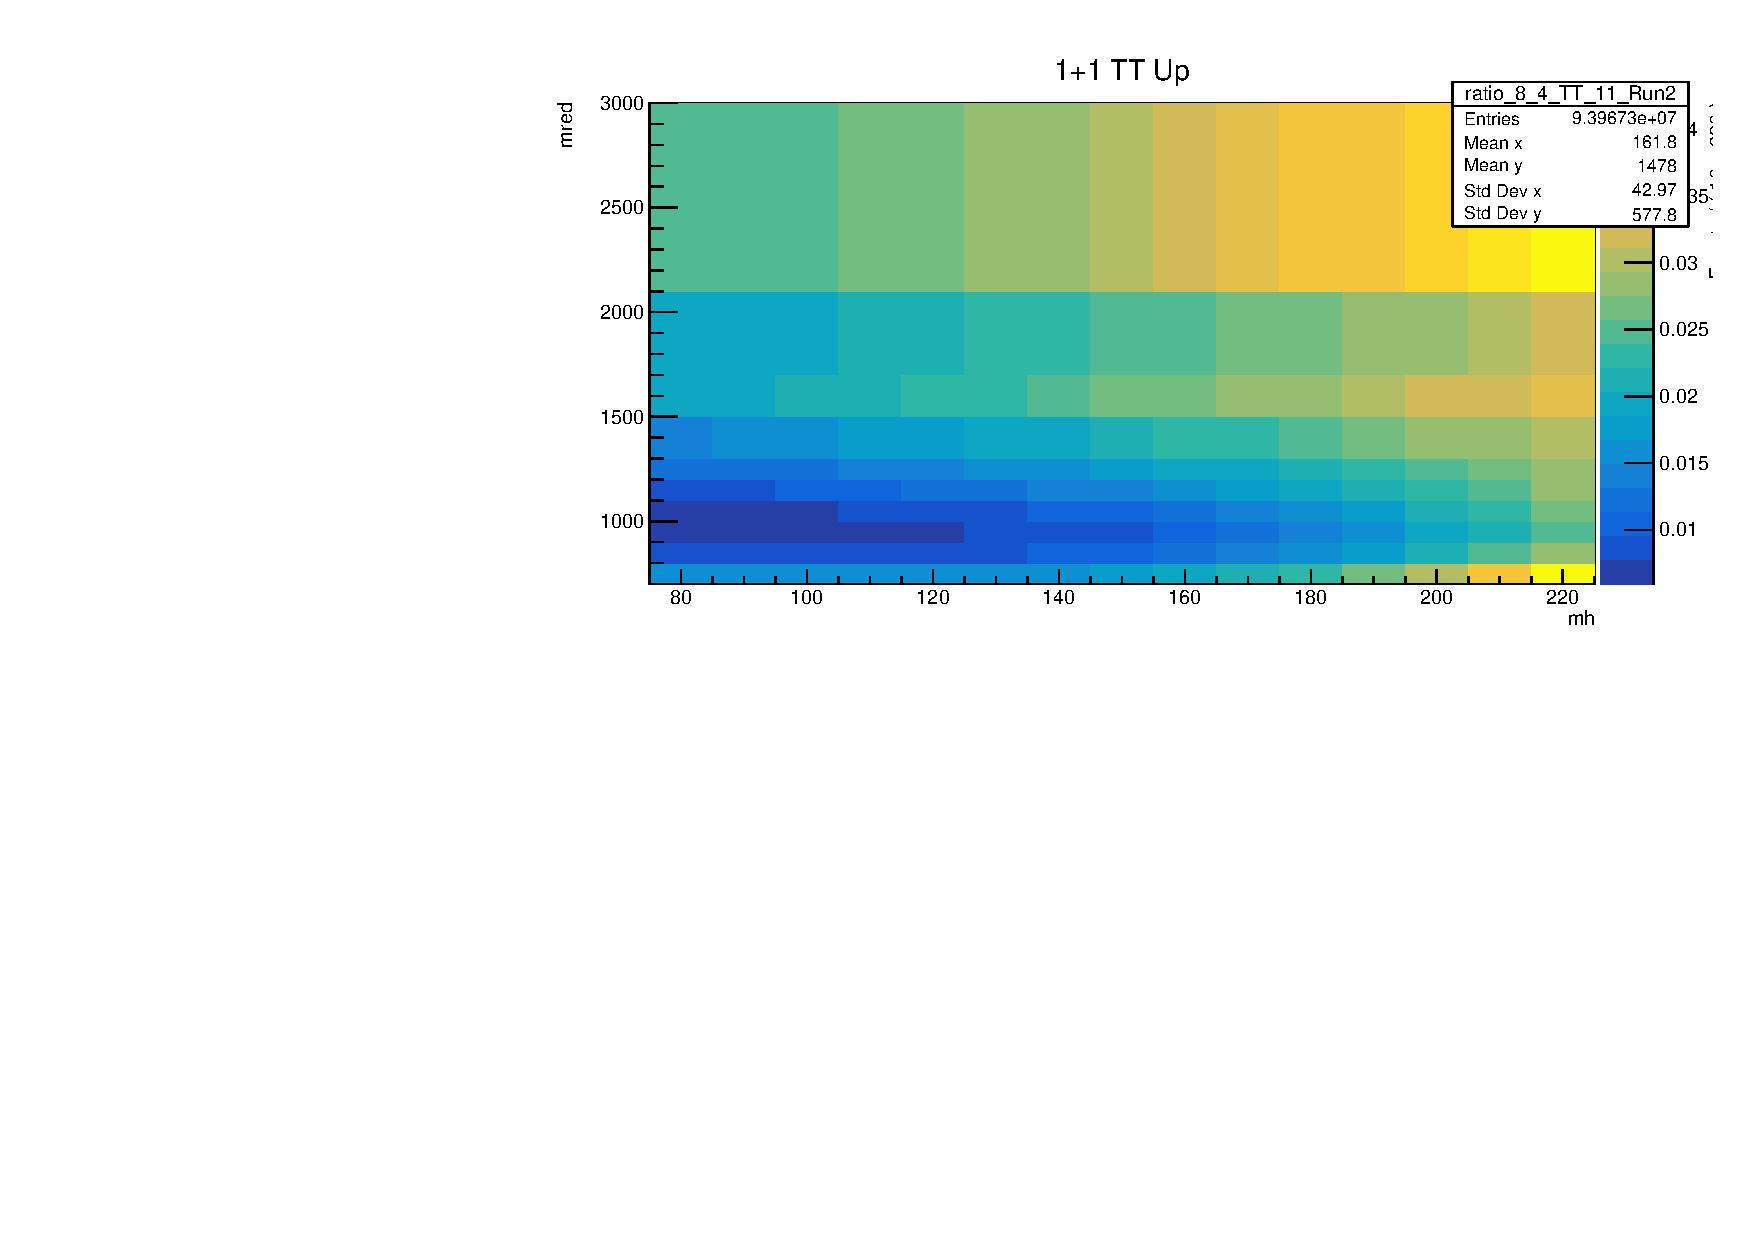
\includegraphics[width=0.5\textwidth]{Figures/TT_up.pdf}
	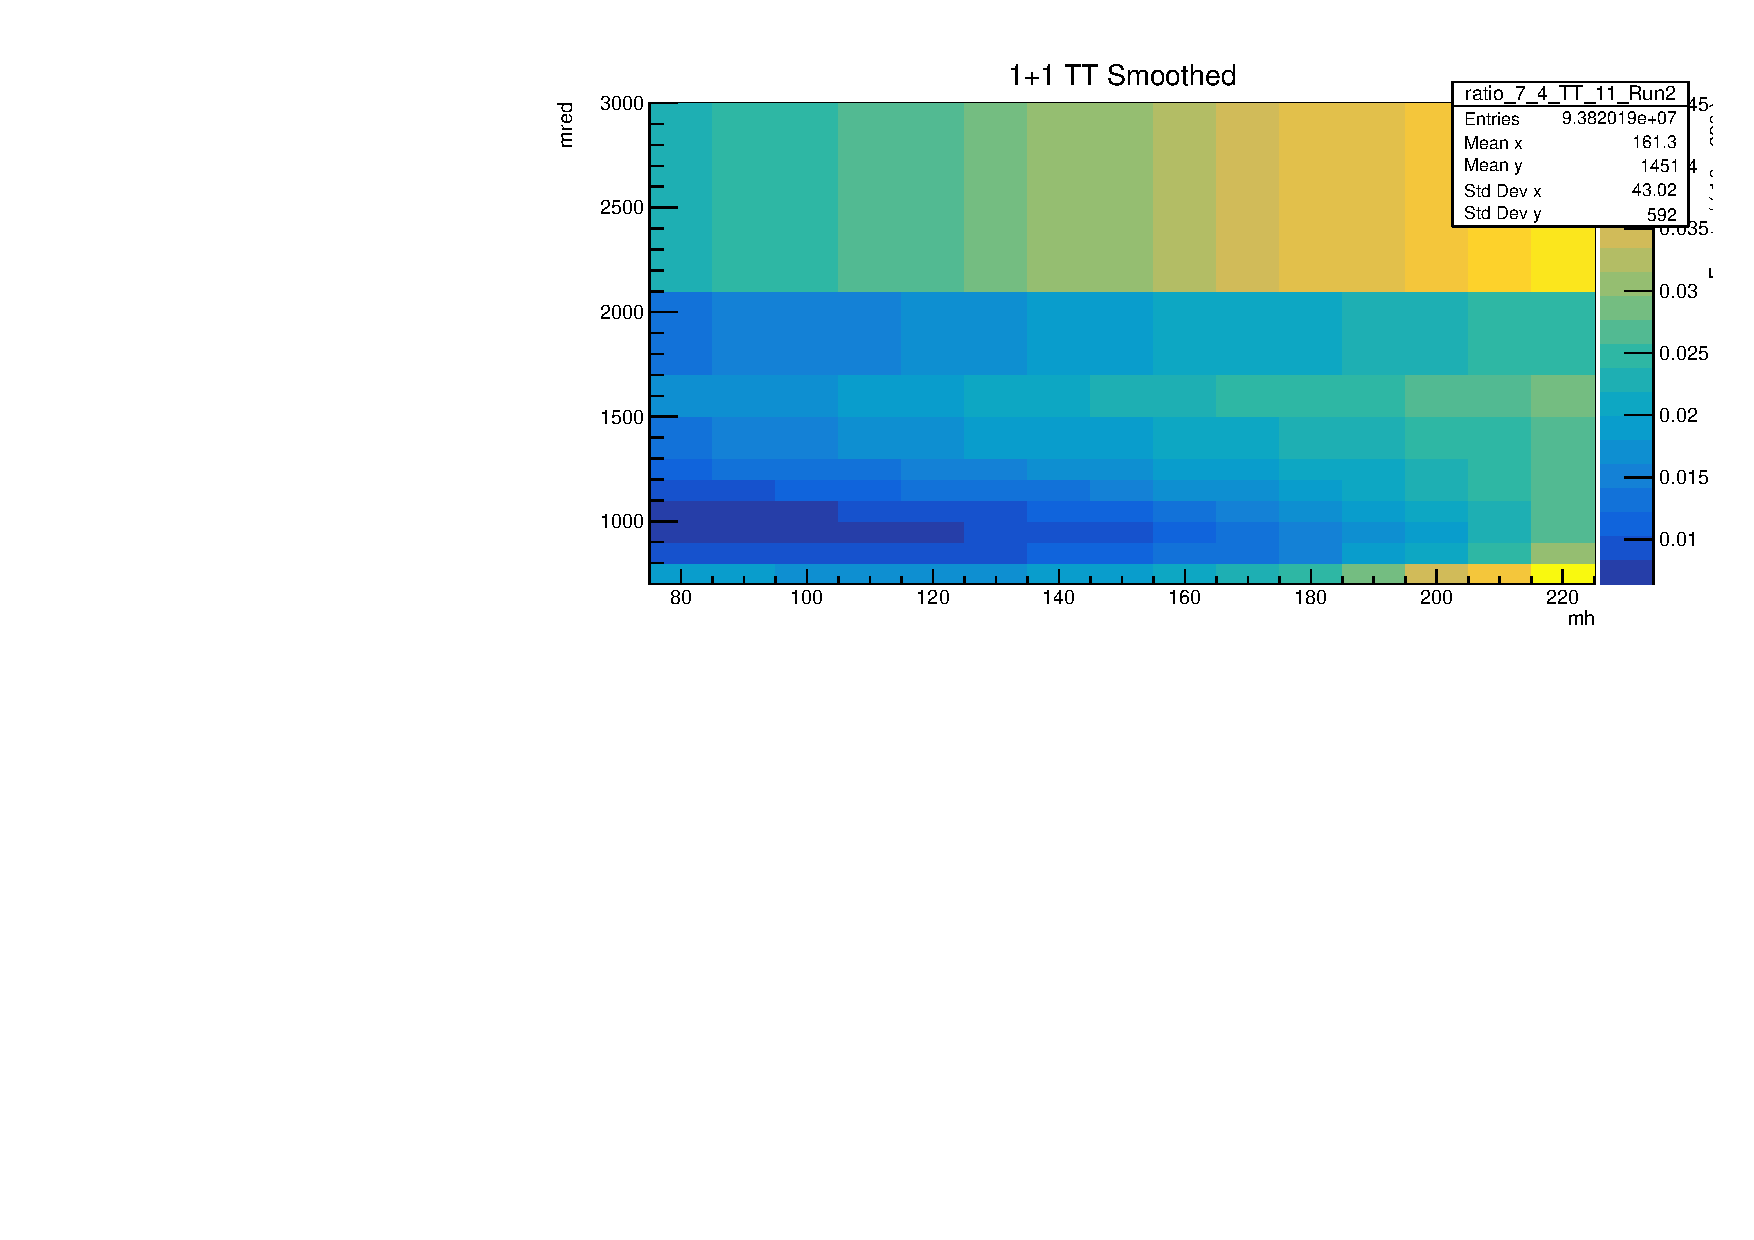
\includegraphics[width=0.5\textwidth]{Figures/TT_smoothed2.pdf}
  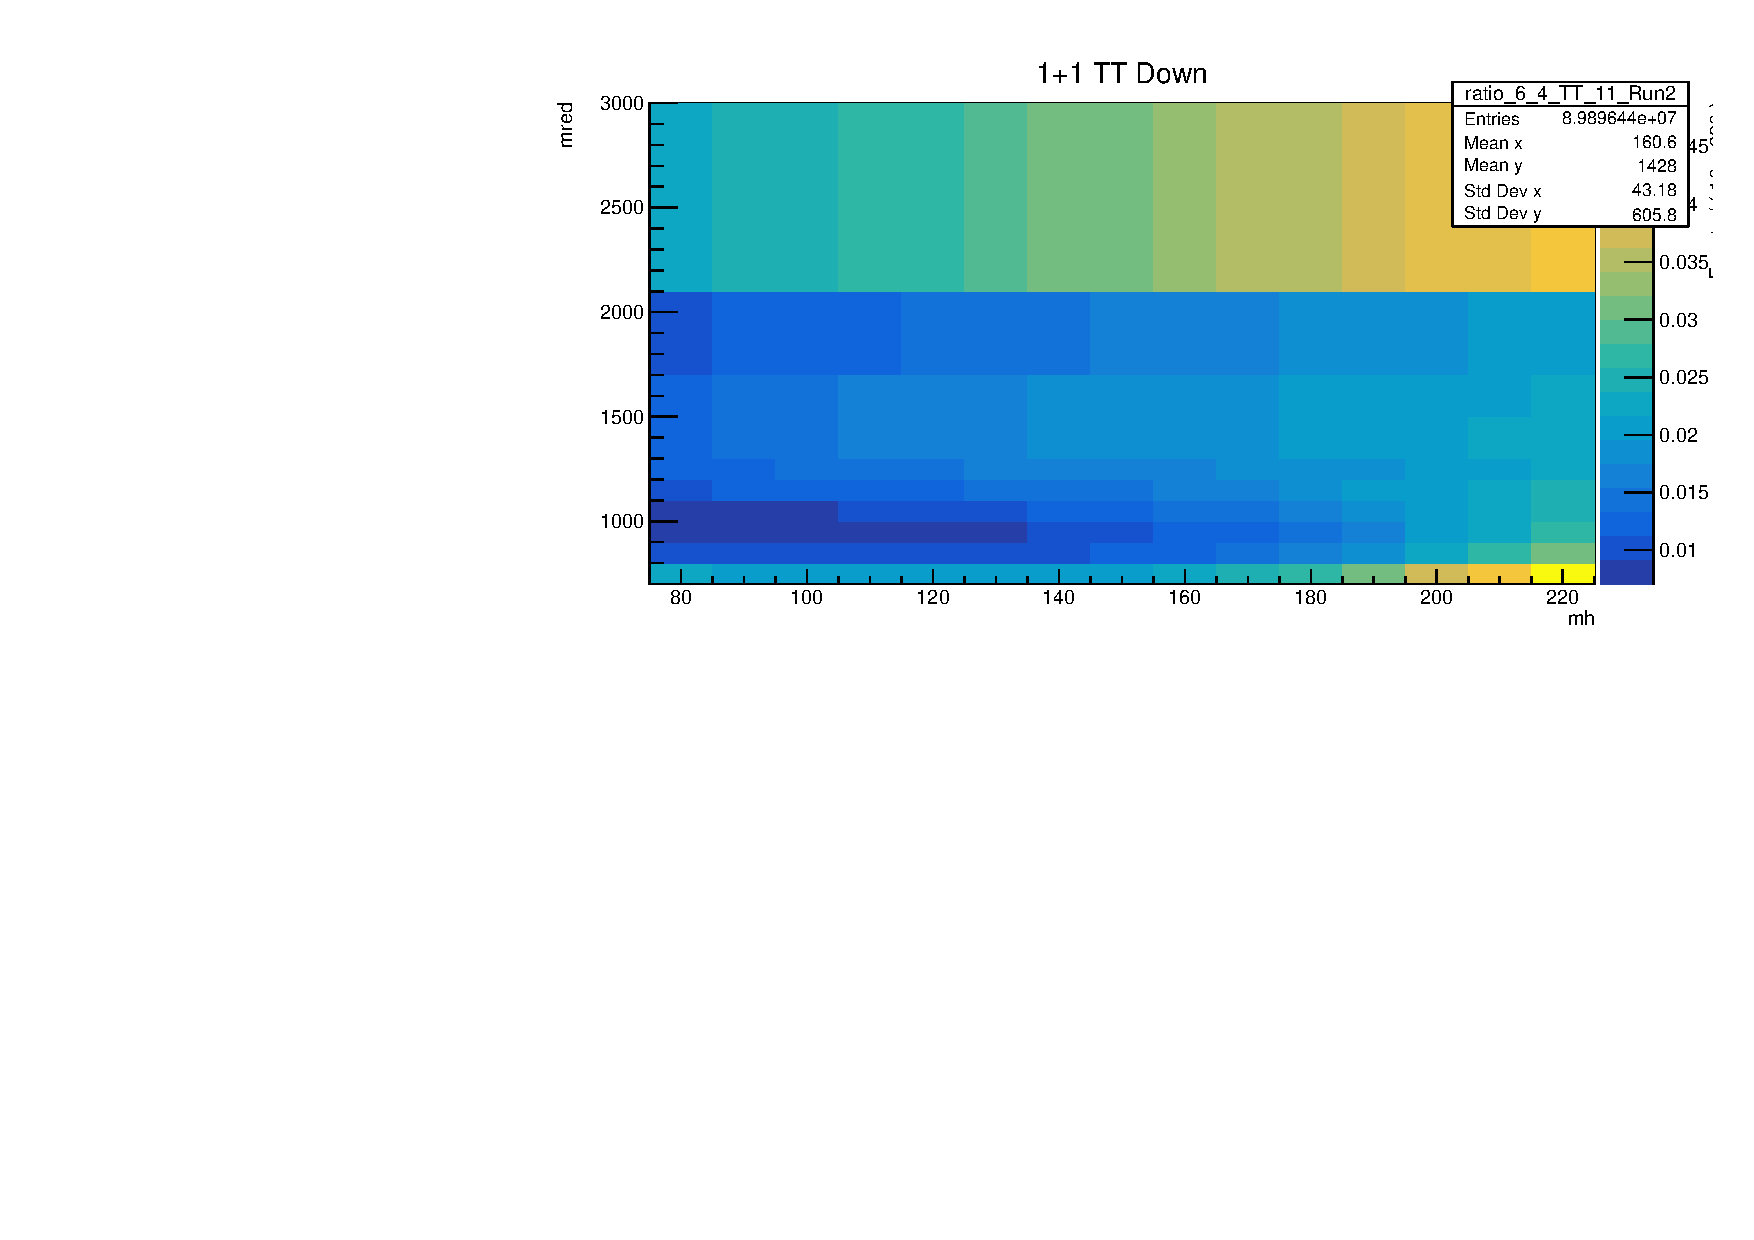
\includegraphics[width=0.5\textwidth]{Figures/TT_down.pdf}
	\caption{KDE bandwidth nominal, up, and down distributions for Tight Tight.}
	\label{fig:KDETT}
\end{figure}
\item \textbf{Prefire Corrections} We apply the recommended 2016/2017 prefire corrections using the nanoAOD tools module to create a nominal correction and$ \pm 1 \sigma$ distributions to be used as a shape based uncertainty.

\end{itemize}
\subsection{$\ttbar$-Tagging Scale Factor Derivation \label{ss:ttbarSF}}
% The single-$\mu$ sample is recorded using a single-muon triggers that select events online based on the muon $\pt$. Candidate events are required to have exactly one muon with $\pt>55 GeV$, satisfying the the tight-ID and miniRelIsolation$<0.1$. To suppress non-$\ttbar$ processes, at least one jet passing the medium working point of the DeepCSV b tagging algorithm is required. In addition, to probe high
% momentum topologies, we require the $\pt$ of the leptonically decaying W bosons, defined as $\vec{p_T}(W) = \vec{p_T}(\mu) + p_{T}^{miss}$ to be greater than 250 GeV. The top/W candidate is the highest pT AK8 jet in the event with $\pt > 200 Gev$, satisfying the criteria discussed in Section X. To further improve the purity, we require the azimuthal angle $\Delta\phi$ between the AK8 jet and the muon to be greater than 2 radians. The purity of the sample in semileptonic tt events is $\sim$70\%; other contributions arise from QCD multijet ($\sim$15\%) and W$+$jets ($\sim$10\%) processes.

The measurement of the t~quark mis-tagging efficiency in data is performed using a tag-and-probe'' method~\cite{Khachatryan:2010xn}. The muon, in combination with the b-tagged jet, is used as
the tag''. In the opposite hemisphere of the event, the jet is
considered as the ``probe jet''.

The total SM  sample is decomposed into three categories based on the spatial separation of the partons from the t~quark decay with respect to the AK8 jet. The merged t~quark'' category includes cases where the three partons and the jet have $\Delta R < 0.6$. The merged \PW~boson'' category includes cases where only the two partons from the \PW~boson decay are within $\Delta R <0.6$ of the jet and the b quark from the top quark decay is outside the jet
cone. Any other topology falls in the ``non-merged'' category. 

The jet mass distributions in simulation of each one of the three categories are used to derive templates to fit the jet mass distribution in data. For a given working point, the fit is done for all three categories simultaneously for both the passing'' and failing'' events. The fit is performed in the range from 50 to 250 Gev with a bin width of 10 Gev. 
 
A number of sources of systematic effects can affect the modeling of the performance of the algorithms in data by the simulation.
These include systematic uncertainties in the parton showering model, renormalization and factorization scales, PDFs, jet energy scale and resolution, $p_{T}^{miss}$\ un-clustered energy, trigger and lepton identification, pileup modeling, and integrated luminosity,
as well as statistical uncertainties of simulated samples.

Parton shower uncertainties are evaluated using samples with the
same event generators but a different choice for the modeling of the
parton showering (i.e. pythia vs. herwig). 
Changes in renormalization ($\mu_{R}$) and factorization ($\mu_{F}$) scales are estimated by varying the scales separately by a factor of two up and down,
relative to the choices of the scale values used
in the sample generation. The uncertainty related to the choice of the
PDFs is obtained from the standard deviation in 100 replicas of the
NNPDF3.0 PDF set~\cite{Ball:2012cx}.
The jet energy scale and resolution are changed within their $\pt$-
and $\eta$-dependent uncertainties, based on the studies presented in
Ref.~\cite{Khachatryan:2016kdb}. Their effects are also propagated to
$p_{T}^{miss}$.
The effect of the uncertainty in the measurement of the un-clustered
energy (i.e., contribution of PF candidates not associated to any of
the physics objects) is evaluated based on the momentum resolution of
each PF candidate, which depends on the type of the
candidate~\cite{Sirunyan:2019kia}.
Uncertainties in the measurement of the trigger efficiency and in the
energy/momentum scale and resolution of the leptons are propagated in the SF extraction.
The uncertainty in the pileup weighting procedure is determined by
varying the minimum bias cross section used to produce the pileup
profile by $\pm$5\% from the measured central value of 69.2 mb
\cite{Sirunyan:2018nqx,Aaboud:2016mmw}.
The limited size of the simulated samples and the size of the data
control samples are also considered.

A logNormal uncertainty of the 10\% is applying to account for possible missing effects on the normalization of the of the three templates obtained from the $\ttbar$ sample. An uncertainty of 50\% is applied to the other subdominant contributions.    

 All sources of systematic uncertainties are treated as nuisance parameters in the fit.  After calculating the efficiencies in data ($\epsilon_{\text{Data}}$)
and simulation ($\epsilon_{\text{Simulation}}$), the SF is
determined as the ratio of $\epsilon_{\text{Data}}$ over $\epsilon_{\text{Simulation}}$.

The $\ttbar$ normalization and the SFs are extracted deferentially in jet $\pt$ for the t quark tagging working point: deepAK8-MD(bb)$>0.90$. The following exclusive jet $\pt$ regions
are considered: 450--600, 600--800, and 800--1200 Gev.